\documentclass[UTF8,fontset=none,a4paper]{ctexart}
\usepackage{fontspec,xeCJK}
\setmainfont{Times New Roman}
\setsansfont{Arial}
\setmonofont{Consolas}[Scale=.82]
\setCJKmainfont{SimSun}[AutoFakeBold=true]
\setCJKsansfont{Microsoft YaHei}
\setCJKmonofont{SimSun}
\usepackage[left=2.5cm,right=2.5cm,top=2.65cm,bottom=2.35cm]{geometry}
\usepackage{amsmath,amssymb,graphicx,booktabs,tabularx,longtable,array}
\usepackage{xcolor,fancyhdr,enumitem,caption,float,tikz,needspace}
\usepackage[hidelinks,unicode]{hyperref}
\usetikzlibrary{arrows.meta,positioning,calc,fit}
\definecolor{navy}{HTML}{173650}
\definecolor{teal}{HTML}{147D85}
\definecolor{pale}{HTML}{F1F5F8}
\ctexset{section={name={第,部分},number=\chinese{section},format=\Large\bfseries,beforeskip=2ex,afterskip=1ex},subsection={format=\large\bfseries,beforeskip=1.7ex,afterskip=.7ex},subsubsection={format=\normalsize\bfseries,beforeskip=1.4ex,afterskip=.5ex}}
\renewcommand{\thesubsection}{\arabic{section}.\arabic{subsection}}
\renewcommand{\thesubsubsection}{\arabic{section}.\arabic{subsection}.\arabic{subsubsection}}
\setcounter{tocdepth}{2}
\setcounter{secnumdepth}{3}
\setlength{\parindent}{2em}
\setlength{\parskip}{.25em}
\setlength{\emergencystretch}{2em}
\renewcommand{\arraystretch}{1.18}
\setlist{nosep,leftmargin=2em,topsep=.3em}
\captionsetup{font=small,labelfont=bf,labelsep=quad,skip=6pt}
\setlength{\textfloatsep}{12pt plus 2pt minus 2pt}
\renewcommand{\topfraction}{.92}
\renewcommand{\bottomfraction}{.85}
\renewcommand{\textfraction}{.08}
\clubpenalty=10000\widowpenalty=10000
\newcommand{\sig}[1]{\texttt{\detokenize{#1}}}
\newcommand{\blocktitle}[1]{\par\medskip\noindent\textbf{#1}\par\smallskip}
\newcommand{\reportfigure}[4]{\begin{figure}[H]\centering\includegraphics[width=#2\linewidth]{#1}\caption{#3}\label{#4}\end{figure}}
\NewDocumentEnvironment{porttable}{+b}{\par\smallskip\noindent\begin{minipage}{\linewidth}\small\begin{tabularx}{\linewidth}{@{}p{.26\linewidth}p{.11\linewidth}X@{}}\toprule 信号或接口 & 方向 & 定义与用途\\\midrule #1 \bottomrule\end{tabularx}\end{minipage}\par\smallskip}{}
\pagestyle{fancy}\fancyhf{}\fancyfoot[C]{\thepage}\renewcommand{\headrulewidth}{0pt}
\IfFileExists{figures/template_header.png}{\AddToHook{shipout/foreground}{\begin{tikzpicture}[remember picture,overlay]\node[anchor=north,inner sep=0pt,yshift=-.65cm] at (current page.north){
\includegraphics[width=6.516cm,height=1.192cm]{figures/template_header.png}};\draw[line width=.75pt] ([xshift=2.5cm,yshift=-2.02cm]current page.north west)--([xshift=-2.5cm,yshift=-2.02cm]current page.north east);\end{tikzpicture}}}{}
\hypersetup{pdftitle={芯绘丹青 基于Ti60 FPGA的十风格视频渲染系统},pdfauthor={},pdfsubject={技术报告 2026年11月3日}}
\begin{document}
\fontsize{11.5pt}{17.5pt}\selectfont
\thispagestyle{empty}
\vspace*{1.4cm}
\begin{center}
{\fontsize{32pt}{44pt}\selectfont\bfseries\textcolor{navy}{芯绘丹青}}\par
\vspace{.45cm}
{\fontsize{17pt}{26pt}\selectfont 端侧实时艺术渲染}\par
\vspace{.3cm}
{\large 基于Ti60 FPGA的十风格视频渲染系统}\par
\vspace{1.15cm}
{\Large\bfseries 技术报告}\par
\vspace{1cm}
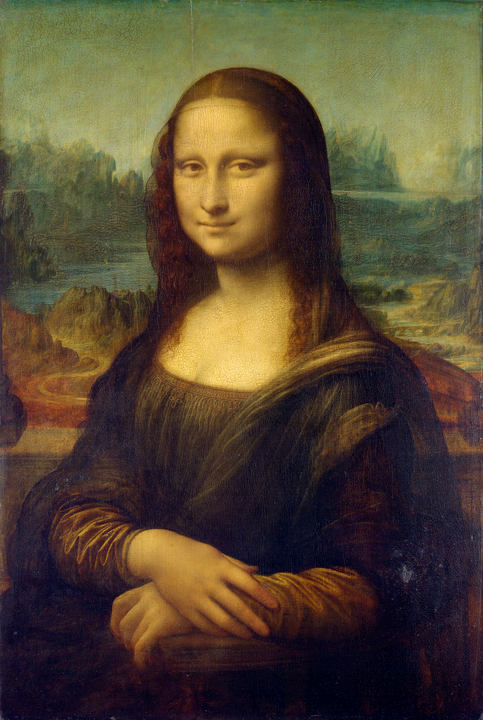
\includegraphics[height=4.2cm]{assets/comparisons/mona_lisa_original.png}\hspace{.25cm}
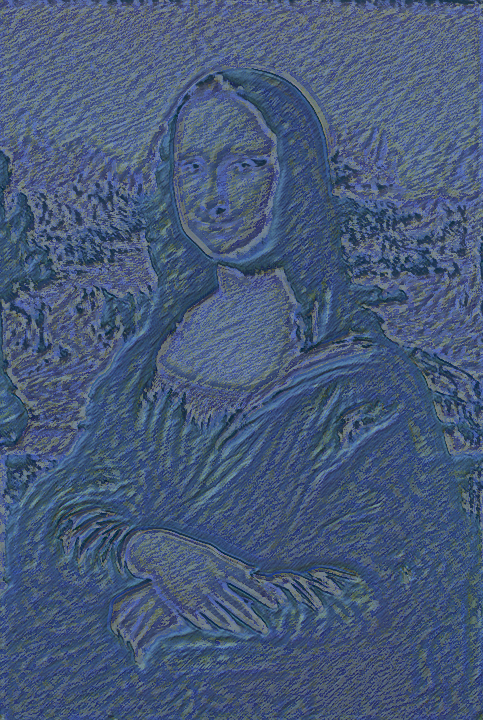
\includegraphics[height=4.2cm]{assets/comparisons/mona_lisa_00.png}\hspace{.25cm}
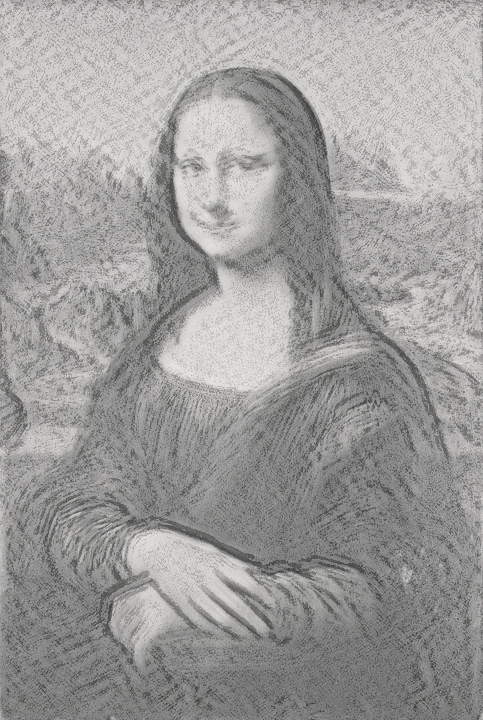
\includegraphics[height=4.2cm]{assets/comparisons/mona_lisa_04.png}\par
\vspace{.2cm}
{\small 原图\hspace{2cm}梵高厚涂\hspace{1.8cm}水墨}\par
\vspace{.25cm}
{\footnotesize 展示图来自当前学生模型的真实整数预测}\par
\vfill
\begin{tabular}{rl}
赛题方向 & AI赋能的“实时绘画”风格化视频渲染\\[5pt]
实现平台 & Ti60F225I3 DemoBoard V4 / SC431HAI\\[5pt]
工程版本 & \sig{camera_art_ten_paint}\\[5pt]
报告日期 & 2026年11月3日
\end{tabular}
\end{center}
\vspace*{.7cm}
\clearpage
\noindent{\fontsize{20pt}{28pt}\selectfont\bfseries\textcolor{navy}{项目速览}}\par
\noindent{\large 摄像头采集 → FPGA风格化 → HDMI呈现}\par
\smallskip

系统将SC431HAI的1080p RAW10视频转换为1280×720 RGB565，写入DDR3后由六通道卷积加速器处理。十组独立风格参数复用一套硬件，RISC-V负责传感器初始化、参数装载、作业与手势控制。网络各层保持720p，显示支持原图、风格图及同源左右对比。

\begin{figure}[H]\centering
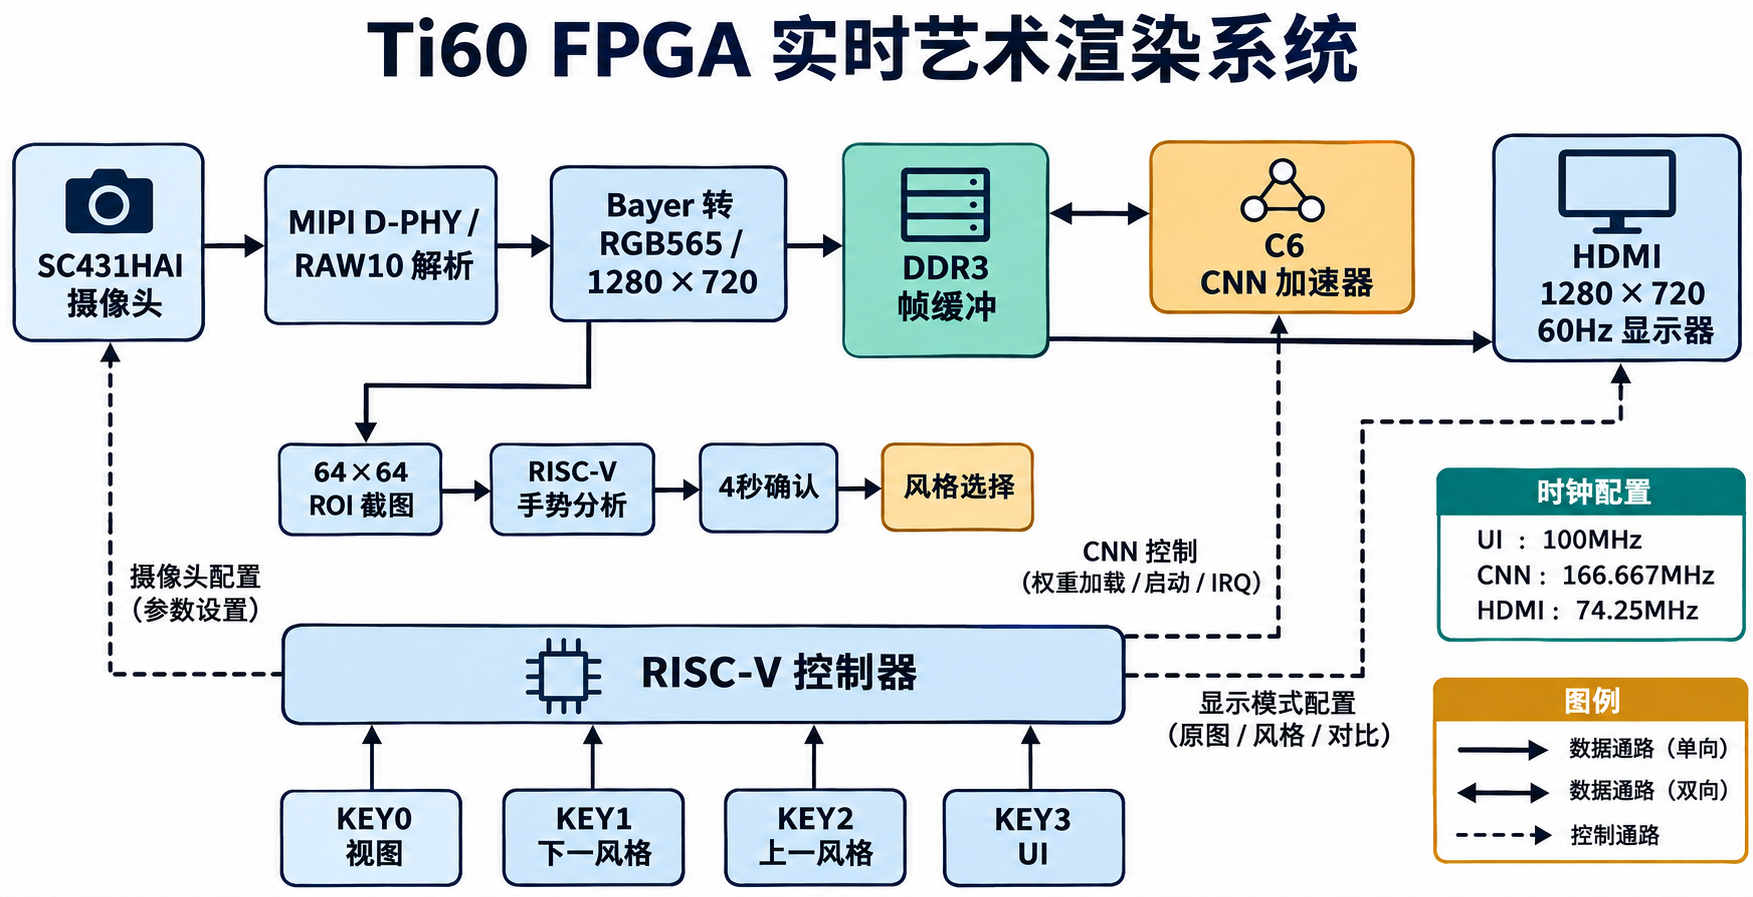
\includegraphics[width=.96\linewidth]{assets/generated/system.png}
\caption{系统总览：数据在DDR中交换，控制经APB传递；板载手势当前使用个人模板。}
\label{fig:system}
\end{figure}

\noindent\begin{tabularx}{\linewidth}{@{}p{.24\linewidth}X@{}}\toprule
核心指标 & 当前实现与证据\\\midrule
图像与显示 & 全1280×720处理；HDMI标准720p60刷新\\
轻量网络 & C6 / RF31；396个卷积权重/风格；十风格ROM 7360B\\
吞吐与资源 & CNN/DMA模型39.085fps；RAM230/256、DSP142/160\\
时序与边界 & setup/hold余量+0.108/+0.026ns；持续板上FPS待量化复测\\\bottomrule
\end{tabularx}
\medskip

\noindent\textbf{一帧流程：}好帧发布 → 锁住源bank → 加载216项参数（需要时）→ 四条带卷积 → 最后DDR写响应 → 安全消隐换帧。三源、三输出槽允许采集、计算和显示重叠。

\smallskip\noindent\textbf{交互方式：}KEY0切换视图，KEY1/KEY2切换风格，KEY3开关UI；在原图/对比界面识别手势0--9，持续四秒确认，原图确认后自动进入风格图。

\smallskip\noindent\textbf{成果范围：}当前bit完成CAD、定点与模块验证；20组名画输出为真实模型预测。免录入通用手势、外部在线权重下载以及持续整机30fps实测仍是后续工作。

\clearpage
\begingroup\small\tableofcontents\endgroup
\clearpage
\section*{摘要}
\addcontentsline{toc}{section}{摘要}
本项目面向端侧实时绘画场景，在易灵思Ti60F225I3平台构建摄像头采集、神经网络风格化与HDMI显示系统。SC431HAI的四lane RAW10经协议检查、Bayer插值和尺寸变换形成1280×720 RGB565图像，经DDR交给六通道轻量卷积加速器。网络由输入投影、四组膨胀DW/PW残差块及有符号RGB输出头组成，各层保持全分辨率。绘画Gram统计、教师引导、局部纹理约束与整数QAT共同用于训练十组独立风格参数。

RISC-V负责摄像头初始化、216项参数装载、作业与中断控制。三源、三输出槽通过完整帧发布和安全消隐提交协调并发，支持原图、风格图及同源对比；按键控制视图、风格和UI，当前板载手势采用个人模板及四秒确认。最终CAD资源为230块RAM10和142个DSP，最小setup/hold余量为+0.108/+0.026ns。完整720p帧的CNN/DMA仿真耗时25.585ms，HDMI输出刷新率为60Hz。

\noindent\textbf{关键词：}FPGA；神经风格迁移；深度可分离卷积；定点量化；RISC-V；视频交互

\section{作品概述}
\subsection{功能与特性}
系统将摄像头视频在本地FPGA上变换为绘画风格画面，主要数据通路不依赖主机推理。图像在DDR中缓存，轻量CNN完成空间纹理和颜色的联合变换，显示支持原图、风格图及同源左右对比。十种参数依次为梵高、浮世绘、剪纸、漫画、水墨、阿什维尔抽象、形体对比、蒙德里安、马赛克及雨夜厚涂。按键提供确定的现场控制；手势以个人模板、投票和四秒保持触发切换。UI显示采集、推理计数及当前风格，便于区分显示刷新与实际新图处理。

\subsection{应用领域}
作品面向互动艺术展示、数字画框、摄像头特效终端及嵌入式视觉教学。本地数据流有利于独立运行和控制视频传输开销，也提供从训练、定点导出、总线调度到FPGA显示的教学实例。手势仅作为交互入口，当前不承担身份识别等需要高可靠判决的任务。

\subsection{主要技术特点}
模型采用六通道DW/PW残差结构，在不下采样的条件下以膨胀卷积扩大邻域。硬件利用分条行缓存、DW三列bank及PW多上下文流水协调RAM和DSP开销。RISC-V与APB组成控制平面，128位AXI承担DDR像素流，避免CPU搬运整幅图像。完整帧发布、最终B响应屏障和安全消隐提交使采集、计算与显示可以并行。INT8权重、逐通道移位和冻结BN折叠将训练模型转换为可逐值核对的整数算术。

\subsection{主要性能指标}
\begin{table}[H]\centering\small
\begin{tabularx}{\linewidth}{@{}lX@{}}\toprule 指标 & 当前结果\\\midrule
图像空间尺寸 & 预处理及CNN为1280×720，显示720p60\\
风格数量 & 10组独立学习参数，共用单套加速器\\
资源与时序 & RAM230/256、DSP142/160；setup/hold +0.108/+0.026ns\\
处理速度 & CNN/DMA模型39.085fps；实际整机持续FPS待复测\\
数值一致性 & 历史50例完整720p、40例小尺寸软件核对；本轮新增20例QAT一致\\\bottomrule
\end{tabularx}
\end{table}

\Needspace{8\baselineskip}
\subsection{主要创新点}
\begin{enumerate}
\item 将全720p六通道网络与分条DW/PW流水共同设计，在有限RAM与DSP下保留逐像素推理。
\item 将帧所有权、参数身份、视图元数据和安全换帧统一管理，使多风格切换与同源对比一致。
\item 建立绘画纹理训练、整数参考、实际固件和CAD报告的对应链，分别评估画质、吞吐和显示刷新。
\end{enumerate}

\subsection{设计流程}
先在Xilinx平台以串口静态图验证协议、DDR和HDMI，再在Ti60平台接入SC431HAI与RISC-V。随后迭代到全分辨率六通道模型，经教师引导、绘画损失及整数QAT训练导出参数，完成RTL数值回归、布局布线与电气核对。每次变更保留旧版本，对新bit单独记录指纹。

\clearpage
\section{系统组成及功能说明}
\subsection{整体介绍}
系统由图像数据平面和软件控制平面组成。数据平面连接摄像头、RAW处理、DDR、CNN和HDMI；控制平面由Sapphire RISC-V、APB寄存器、按键和手势状态机构成。\sig{video_system_720}在100MHz UI域组织帧池、作业与DDR仲裁，通过异步FIFO与166.667MHz CNN域、74.25MHz显示域交换数据。摄像头字节时钟来自D-PHY，可能在低功耗期间停止，因此不直接跨域采样多位包头。

\begin{table}[H]\centering\small
\caption{模块与主要源码对应}
\begin{tabularx}{\linewidth}{@{}p{.27\linewidth}X@{}}\toprule 功能 & 主要源码\\\midrule
PPI与CSI解析 & \sig{csi_ppi_bridge_recover.sv}\\
RAW预处理 & \sig{camera_bayer_720.sv}\newline \sig{camera_pack_720.sv}\\
源帧与作业管理 & \sig{camera_frame_writer_720.sv}\newline \sig{source_frame_pool.sv}\newline \sig{video_job_control.sv}\\
分条DMA与跨域 & \sig{video_tile_engine_async.sv}\newline \sig{video_cnn_async.sv}\\
卷积及参数 & \sig{full_dw3x3.sv}\newline \sig{full_pointwise.sv}\newline \sig{full_parameter_bank.sv}\\
显示及UI & \sig{frame_reader.sv}\newline \sig{video_raster60.sv}\newline \sig{fps_overlay60.sv}\newline \sig{tmds_hdmi60.sv}\\
CPU及交互 & \sig{video_control_apb_fast.sv}\newline \sig{style_keys47.sv}\newline \sig{gesture_snapshot.sv}和C固件\\\bottomrule
\end{tabularx}
\end{table}
除特别注明外，摄像头解析、帧池、作业、DDR用户接口及APB均使用100MHz的clk和高有效reset；CNN使用166.667MHz的\sig{fast_clk}，扫描使用74.25MHz像素时钟。本文将同组总线适当合并列出，低电平命名的外部复位在顶层转换，不与内部reset混用。

以下接口表列出主要模块边界，不重复展开全部诊断端口及厂商DDR PHY。方向均相对该节模块；有效/就绪型流仅在valid与ready同时有效时前进，无ready的摄像头输入必须持续接收。

\subsection{硬件系统介绍}
\subsubsection{平台与电气接口}
系统采用Ti60F225I3 DemoBoard V4及demo10配套SC431HAI排线模组，沿用板载DDR3、USB串口和HDMI，未增加自制机械或供电结构。板级依据为20261012版原理图\cite{board}；采集参考V7，对照V9的Bayer与数据延迟处理\cite{demo}，未改原demo。
\begin{table}[H]\centering\small
\caption{外设连接与电平约束}
\begin{tabularx}{\linewidth}{@{}p{.22\linewidth}p{.18\linewidth}X@{}}\toprule 接口 & 配置电平 & 连接与实现约束\\\midrule
MIPI专用RX & 1.2V & Bank2A/2B；配套模组接J4，J2/J3均2--3\\
摄像头控制 & 3.3V & SCL D12、SDA B14开漏；C12模组RESET高有效\\
四按键 & 3.3V输入 & KEY0--3依次C4、P14、N14、A3，低有效\\
板载USB串口 & 3.3V & R4 RX、R14 TX；J8不是UART接线座\\
DDR3 & 1.5V & 保留原板DDR PHY、终端及OE绑定\\
HDMI串化侧 & 1.8V & Bank3A，使用现有板级TMDS电路\\\bottomrule
\end{tabularx}
\end{table}
电气签核逐项检查79个实际端口、12组Bank、方向、I/O标准及DDR数据/OE绑定，与CAD时序检查相互独立。用户已确认J4和跳线接法；实际电源电压、连接器状态和温升仍须实板测量，数字审查不代替物理测量。


\blocktitle{板级连接与内部总线的分工}
图\ref{fig:board-direction}区分电气接口与片内数据接口。DDR引脚侧为16位双沿数据总线，用户侧则是100MHz、128位AXI，二者通过厂商控制器转换；不能把AXI位宽或UI频率直接套到外部DQ上。MIPI只承担输入，HDMI只承担输出，GPIO控制信号与高速差分信号分别使用对应Bank供电。
\begin{figure}[H]\centering
\begin{tikzpicture}[x=1cm,y=1cm,every node/.style={font=\small,align=center},
box/.style={draw=navy,rounded corners=2pt,minimum height=.85cm,text width=3.1cm},
arr/.style={-{Stealth},thick,draw=teal}]
\node[box] (cam) at (0,1.3) {J4摄像头模组\\MIPI RX / 控制GPIO};
\node[box] (key) at (0,-1.3) {四按键 / 板载USB\\输入 / 串口诊断};
\node[box,minimum height=3.6cm,text width=3.3cm] (fpga) at (5,0) {Ti60F225I3\\[4pt]D-PHY / DDR PHY\\RISC-V / CNN\\TMDS编码及串化};
\node[box] (ddr) at (10,1.3) {U12 DDR3\\DQ / DQS双向};
\node[box] (hdmi) at (10,-1.3) {HDMI连接器\\TMDS输出};
\draw[arr] (cam.east)--node[above,font=\scriptsize]{RAW10}(fpga.west|-cam.east);
\draw[arr] (fpga.west|-0,.6)--node[below,font=\scriptsize]{I²C / RESET}(0,.6)--(cam.south);
\draw[arr] ([yshift=2mm]key.east)--node[above,font=\scriptsize]{按键输入}([yshift=2mm]fpga.west|-key.east);
\draw[arr] ([yshift=-2mm]fpga.west|-key.east)--node[below,font=\scriptsize]{UART诊断}([yshift=-2mm]key.east);
\draw[arr,<->] (fpga.east|-ddr.west)--node[above,font=\scriptsize]{数据 / 选通}(ddr.west);
\draw[arr] (fpga.east|-hdmi.west)--node[above,font=\scriptsize]{视频 / 时钟}(hdmi.west);
\end{tikzpicture}
\caption{板级接口方向示意，省略电源和所有单根管脚。配置电平以表格和79端口审查清单为准。}
\label{fig:board-direction}
\end{figure}
摄像头I\textsuperscript{2}C不是推挽高低输出。固件写入\sig{scl_release/sda_release}，置1表示高阻释放，由模组接口上拉形成高电平；置0才驱动低电平，并从输入端读回总线状态。板上配套模组的3.3V控制兼容性不能外推到裸传感器。复位信号的内部名称含\sig{sensor_reset_n}，但连接模组时须结合顶层极性变换判断，不能单凭后缀认定引脚低有效。

DDR必须在PLL锁定、PHY复位释放和校准完成后接收图像访问；校准失效时撤销源帧有效性。HDMI发送使用板上既有耦合、偏置和保护电路，保持原配置与方向。

\subsubsection{摄像头接收与RAW预处理}
\blocktitle{作用}
将四lane CSI-2 RAW10包恢复为可发布的RGB565帧。\sig{csi_ppi_bridge_recover}将字节及SoT等状态形成44位记录，经512深异步FIFO送入UI域，保持数据与状态原子对应。解析器检查包头、ECC/CRC、字节数与帧长度，错误帧不发布。
\begin{porttable}
四lane PPI字节及状态 & 输入 & 32位数据与各lane有效、同步及SoT，来自D-PHY RX\\
\sig{vs/hs/valid/raw} & 输出 & 帧、行、样本有效及40位RAW10四样本\\
\sig{packet_error/overflow} & 输出 & 包错误与FIFO溢出，影响整帧有效性\\
\sig{frame_start/end/bad} & 输出 & 预处理后边界与坏帧标志，供打包及手势旁路\\
\sig{pixels[31:0]} & 输出 & 两个RGB565像素，低16位为较早的左像素\\
\end{porttable}
传感器配置为1920×1080四lane RAW10，每行2400字节，每五字节恢复四个10位样本。Bayer模块以邻行、邻列插值补齐颜色，再按约$x=\lfloor3u/2\rfloor$、$y=\lfloor3v/2\rfloor$映射形成1280×720全视野输出，RAW高八位量化为RGB565。尺寸变换在CNN之前进行；风格网络内部不再减半分辨率。帧尾排空插值与打包流水，核对像素数，避免漏掉最后一行。


\blocktitle{协议解析状态与错误边界}
接收器分为字节域记录、UI域lane队列和协议状态机三层。每条lane的小队列消化到达差异，只有需要的lane数据齐备才弹出对应字节。其主要状态为\sig{WAIT_SOT}、\sig{HEADER}、\sig{PAYLOAD}、\sig{CRC}：等待同步、识别4字节包头、累计指定长度负载，再比较CRC。短包携带帧边界，长包携带RAW行。当前范围是VC0、四lane、每次HS传输一个CSI包，RAW10长包datatype为\sig{0x2B}，行word count固定2400。

ECC检查采用检测后拒绝策略，包括可纠正单比特错误也不自动修复。CRC错误、缺行、长度不符或包中断均使当前帧失效。仅在所有lane队列已空、处于等待SoT且该记录不含数据或同步时，将孤立SoT状态记为软事件；这不会跳过随后的帧边界、ECC、CRC和尺寸检查。异步FIFO溢出属于保持故障，需要复位恢复。由此将“传输恢复”与“接受一幅好图”分开。

\blocktitle{RAW10解包、颜色与位置一致性}
每组负载字节记为$b_0,\ldots,b_4$，四个RAW样本恢复为
\[
p_i=(b_i\ll2)\;|\;((b_4\gg2i)\,\&\,3),\quad i=0,1,2,3.
\]
输出\sig{raw[39:0]}由低到高放置$p_0$到$p_3$。预处理取各样本高八位，两拍处理四个RAW样本；两条行缓存与横向历史组成3×3窗口。以BGGR为例，蓝色位置保留中心B，四个正交邻点平均得到G，四个对角邻点平均得到R；绿色位置依据行列奇偶选择水平或垂直邻点恢复R/B。Bayer模式在帧起点锁存，邻域数据、行列奇偶与有效标志一起延迟。

尺寸变换保留每组三个RAW坐标中的前两个，对应源坐标序列$0,1,3,4,\ldots$。最后输出坐标映射到RAW的1918列、1078行，仍可取得右、下邻点；左、上边界使用reflect101。它是插值后的取样，不是通用抗混叠缩放滤波器，也不是把640×360重复放大。图像偏绿需要分别检查Bayer相位、通道排列及照明白平衡，单改风格权重不能修复输入颜色错误。

\begin{table}[H]\centering\small
\caption{相邻模块的数据布局契约}
\begin{tabularx}{\linewidth}{@{}p{.24\linewidth}p{.21\linewidth}X@{}}\toprule
边界 & 位宽/布局 & 推进与帧尾条件\\\midrule
D-PHY→PPI FIFO & 44位：状态12＋数据32 & 数据与状态同一记录跨域\\
CSI→Bayer & 40位，4个RAW10 & \sig{valid}限定样本，\sig{vs/hs}限定帧行\\
Bayer→打包 & 32位，2个RGB565 & \sig{pixel_valid}一次推进2像素\\
打包→DDR writer & 179位记录 & 独立EOF；不以最后像素代替好帧结束\\
DMA→CNN & 24位，R在低8位 & valid/ready同拍握手才消费\\
显示FIFO→raster & 16位RGB565 & 有效区逐像素读取，无数据则计欠载\\\bottomrule
\end{tabularx}
\end{table}

\subsubsection{DDR写入与源帧池}
\blocktitle{作用}
将无背压的摄像头像素流与受仲裁影响的DDR分离。128位字由低至高排列8个RGB565像素，行stride为2560B，每帧1843200B，即115200个128位字。写入记录使用17位字索引，避免超过65535字后回绕。
\begin{porttable}
\sig{fifo_data[178:0]} & 输入 & 含帧号、字索引、坏帧及独立EOF的像素记录\\
\sig{allocate/allocation_ack} & 双向 & 写帧前申请空闲bank并获得编号\\
\sig{AW/W/B} & 双向 & 写地址、128位数据、最终响应；B错误作废本帧\\
\sig{publish/abort_capture} & 输出 & 发布完整好帧或丢弃，半帧不能成为有效源\\
\sig{claim/release} & 双向 & 引擎领取并锁住源bank，使用后释放\\
\end{porttable}
\sig{source_frame_pool}管理4、6、8MiB三个源bank，轮流承担采集、最新完整帧及引擎锁定帧。一个bank不能同时被覆盖和读取。推理落后时允许新好帧替换未领取旧帧，并显式累计跳过数；持续采集不等于每帧都已经推理。


\blocktitle{DDR中的地址安排}
所有bank以2MiB为槽跨度，一幅720p RGB565占用约1.758MiB，剩余空间不作为下一帧有效像素。行主序、无行间padding，坐标$(x,y)$对应字节地址
\[
A(x,y)=A_{\rm bank}+2560y+2x.
\]
\begin{table}[H]\centering\small
\caption{六个图像槽的地址及所有权}
\begin{tabularx}{\linewidth}{@{}p{.23\linewidth}p{.31\linewidth}X@{}}\toprule
图像槽 & 基地址 & 谁能写、何时释放\\\midrule
输出0 / 1 / 2 & \sig{0x000000 / 0x200000 / 0xA00000} & 引擎写；前台槽需显示commit ACK后释放\\
原图0 / 1 / 2 & \sig{0x400000 / 0x600000 / 0x800000} & 摄像头写；CNN领取后锁至作业结束\\\bottomrule
\end{tabularx}
\end{table}
打包记录的位定义为\sig{[178]EOF}、\sig{[177]bad}、\sig{[176:145]frame_id}、\sig{[144:128]word_index}和\sig{[127:0]pixels}。四拍双像素合成一个128位词，先来的像素处于低位。EOF是独立记录，其index应等于115200；它证明帧边界已到达，而不是只证明缓存中曾出现足够像素。

\blocktitle{写入状态机和发布屏障}
\sig{camera_frame_writer_720}经过IDLE、ALLOCATE、ALLOC\_WAIT、WRITE和RESP。检测到新帧首词先申请bank，收到allocation ACK再开始写；WRITE分别记录AW和W是否握手，允许二者不同拍完成。进入RESP后等待真正B响应，成功后才读取下一记录。EOF只有在精确词数、连续index、同frame\_id、无bad且此前B全部成功时触发publish。写数据握手完成不能提前当作帧可用。

源池用\sig{capture_owned}、\sig{engine_owned}与\sig{latest_valid}表述所有权。空闲槽的选择同时排除三个占用角色。若claim与新publish同拍，旧latest交给引擎，新好帧成为latest；引擎仍读取旧帧，采集不会覆写它。未领取的latest被下一好帧替代时累加skipped计数。分配失败或FIFO积压引起的坏帧与这种主动舍弃必须分开统计。

这种安排允许推理速度暂时落后，同时保持读取帧完整。代价是系统倾向处理最新可用帧，不能承诺输入每一帧都被推理；实际是否发生跳帧需读取运行计数。

\subsubsection{作业控制与输出槽}
\sig{video_job_control}负责源帧及输出槽所有权，APB与系统集成逻辑锁存作业风格和视图。忙中仅保留最新用户请求，不改变正在计算的身份。三个输出槽位于0、2、10MiB，轮流承担计算、待提交和前台，最多维护两项完整输出队列。
\begin{porttable}
\sig{start/raw_mode} & 输入 & 作业启动与原画标志，上层先检查源帧与权重\\
\sig{claim/claim_ack} & 双向 & 领取完整源帧，并返回锁定的source\_frame\\
\sig{engine_start/done/error} & 双向 & 启动引擎；done晚于最后DDR B成功响应\\
\sig{output_bank} & 输出 & 锁定的目的槽；源地址由源池bank换算\\
\sig{commit/commit_ack} & 双向 & 安全消隐提交与显示确认，ACK后释放旧前台\\
\end{porttable}
左原右风格在CNN内已经对齐的原RGB支路上，以全局$x<640$选择原图，右侧选择风格结果，二者来自同一源帧与坐标；不将“最新原图”叠到旧风格帧。每个输出槽保存视图及风格元数据，前台身份只在commit ACK后更新。


\blocktitle{计算完成与显示完成为什么分开}
计算完成表示全部输出已写入DDR，显示完成表示显示端已经安全采用这一bank。若把两者串行绑定，25.6ms的计算还可能等待下一次16.67ms显示边界。当前控制器在计算结束后立即释放源帧并将结果排队，下一作业可在另一个空闲输出槽启动，显示端独立消费完整队列。

作业状态机为IDLE→CLAIM→RUN。IDLE检查空闲输出槽和队列容量；CLAIM等待源池回传锁定的bank/frame\_id；RUN发出一次engine\_start并等待done或error。error优先于同拍done，失败作业释放源但不入显示队列。队列最多两项，且旧前台占用独立保存；显示reader提前改变观察用的front\_bank并不能释放旧槽。

\begin{figure}[H]\centering
\begin{tikzpicture}[every node/.style={font=\small,align=center},n/.style={draw=navy,rounded corners,text width=2.7cm,minimum height=1cm},a/.style={-{Stealth},thick,teal}]
\node[n] (a) at (0,0){空闲输出槽\\领取完整源帧};
\node[n] (b) at (3.9,0){RUN\\计算并写DDR};
\node[n] (c) at (7.8,0){READY队列\\最后B已成功};
\node[n] (d) at (11.7,0){FRONT\\显示安全ACK};
\draw[a] (a)--(b);\draw[a] (b)--(c);\draw[a] (c)--(d);
\draw[a] (d.south)--++(0,-.7)-|node[pos=.25,below]{下一次换帧ACK后，旧前台才回收}(a.south);
\end{tikzpicture}
\caption{输出槽生命周期。源帧锁在计算结束时释放，旧显示槽锁在下一次安全换帧ACK时释放。}
\label{fig:ownership}
\end{figure}
对比模式在计算结果形成时合成，不需要显示端额外再读一幅原图。原RGB由独立FIFO保存到对应CNN增量到达，两支路都有效才接受下游ready；因此背压不会把第$n$个原像素与第$n+1$个风格像素相加。分条坐标加上origin恢复全局位置，左半边原图与右半边风格的分界始终是全图第640列。

\subsubsection{分条DMA与总线仲裁}
\sig{video_tile_engine_async}将720p拆为四条：每条有效320列，左右各16列halo，实际输入352×720。四条各输出320×720，拼回完整921600像素。halo只提供邻域，不作为重复像素发布；边界按全局图像坐标作reflect101处理。
\begin{porttable}
\sig{clk/fast_clk/reset} & 输入 & UI100MHz与CNN166.667MHz，原子FIFO及握手跨域\\
\sig{start/style/raw_mode} & 输入 & 作业启动与模式标志，启动时锁存\\
\sig{cfg_valid/address/data} & 输入 & 配置写入；由cfg\_ready反馈接收状态\\
\sig{AR/R}\newline \sig{AW/W/B} & 双向 & 30位字节地址、128位数据，核对响应和RLAST\\
\sig{busy/done/error/cycles} & 输出 & 作业状态与UI域周期计数\\
\end{porttable}
引擎采用突发读，两组128位写打包槽重叠拼包和AXI事务。读仲裁优先响应同时请求的显示读取，授予事务保持至RLAST。写信用由真实B响应释放，不以W通道完成代替DDR写完成。背压期间保持地址、数据与valid，异常响应不先写入有效显示FIFO再报错。


\blocktitle{四条带的几何关系}
第$k$条有效列为$320k\ldots320k+319$，输入原点为$320k-16$。四条输入横坐标范围分别是$[-16,335]$、$[304,655]$、$[624,975]$和$[944,1295]$。只保留本条局部$x=16\ldots335$的结果。31×31感受野的半径是15，16列halo覆盖邻域并留出对齐余量。

每一层按全局图像边界处理reflect101，不能将条带接缝误当作独立图像边缘。条外填充位置不作为最终输出；极左/右边界的镜像取样由算子层的全局有效区域逻辑完成。逻辑计算像素量为$4\times352\times720=1013760$，比完整图多10\%；实际DDR读流量还受256B缓存块对齐及重取影响，不能只按10\%估算总线开销。

\blocktitle{读缓存、写打包与错误排空}
读地址按256B对齐，每个突发16拍、每拍128位，装入16词局部缓存；按像素$x$的高位选缓存块、低位选词和16位lane。单个突发不跨4KiB边界。显示与CNN使用读仲裁器，授予后维持所有权至RLAST，避免两主机混收一条响应。

输出按8个RGB565像素合成一词，两个打包槽轮流承担“正在发送”和“正在拼下一词”。只有B响应退休该槽；W完成但B未回时槽仍占用。引擎一笔写与摄像头一笔写可由\sig{axi_write_pair}形成总共两笔在途，所有者队列按固定ID响应顺序路由B。它不是无限发射的多ID写DMA。

遇到RRESP错误、RLAST位置错误或BRESP错误，停止接受新的有效输出，先排空已获总线接受的事务，随后报告error。四条全部结束、保留像素数等于921600、写队列为空且最终B成功才发done；任何单条done都不能发布半幅图。

\blocktitle{带宽和算力分别预算}
仅按有效RGB565字节，30fps采集、30fps推理读写及60Hz显示至少需要
\[
1.8432\,{\rm MB}\times(30+30+30+60)=276.48\,{\rm MB/s}.
\]
该式不含halo、缓存重复读取、DDR刷新和仲裁空洞。128位100MHz UI的每方向理论数据峰值为1.6GB/s，但单拍写响应、行切换和共享存储器会显著降低有效率，必须用真实并发计数验证。卷积名义运算量为396 MAC/像素，包含halo约4.0145亿MAC/帧，30fps约120.44亿MAC/s；这解释了为何需要流水、并行和片内复用，不能只看权重文件很小便认定容易实时运行。

\subsubsection{CNN卷积与参数存储}
\sig{full_dw3x3}执行六通道独立3×3膨胀卷积，多行缓存保存历史，列地址分为三个bank，内部位置并行读取三tap。反射边界遇到bank冲突时用第二读阶段补齐，再进入乘加，不复制整份历史以增加端口。\sig{full_pointwise}执行1×1投影、通道混合与有符号输出头，采用两输出通道lane、四像素上下文重叠计算。context标签随流水传递，按接收顺序退休，保持像素顺序。
\begin{porttable}
\sig{in_data/valid/ready} & 双向 & DW输入48位六通道uint8；PW依CIN参数确定\\
\sig{in_skip/in_inside} & 输入 & 同像素残差及全局有效区域标志\\
\sig{out_data/valid/ready} & 双向 & 中间六通道uint8；head为三个有符号16位值\\
\sig{origin_x/start} & 输入 & 条带全局横向原点和初始化，决定图像边界\\
\sig{cfg_valid/address/data} & 输入 & 权重、偏置、逐通道移位的原子配置\\
\end{porttable}
\sig{full_parameter_bank}按layer、kind、item选中参数；APB控制器检查范围与装载顺序。十组风格只保留一个活动工作集，共用计算核。增加风格主要增加ROM和目录，仍有存储与控制开销，不能说风格数完全不影响资源。


\blocktitle{DW：用行历史换取空间邻域}
DW对每个通道独立计算$z_c(x,y)=\sum_{i,j}w_{c,i,j}h_c(x+di,y+dj)+b_c$，$i,j\in\{-1,0,1\}$。历史RAM按条带宽度配置，只保存计算窗口所需的行，避免缓存整幅六通道特征图。三个列bank允许一个阶段读取一组三个横向tap，乘加结果再按行组归并；边界镜像发生端口冲突时补读而不产生错误重复值。

窗口形成、地址计算、同步RAM读出、乘积和加法树分别寄存，局部行基址提前计算，缩短“坐标→bank→RAM地址→乘加”的组合链。每次新条带start重置有效历史及坐标，不能借用上一条残留。RAM旧值存在不等于有效窗口存在，必须同时检查inside和行列有效条件。

\blocktitle{PW：通道维复用与有序输出}
PW计算$z_o=\sum_{c=0}^{C_{\rm in}-1}w_{o,c}h_c+b_o$。两条输出lane并行处理两个输出通道，四组context保存不同像素的输入、中间累加和完成状态，在乘加等待期间处理其他context。结果按输入顺序退出；不能按哪个context先算完就先输出，否则后续行缓存的空间坐标会错位。输入端ready只在存在可用context且下游容量允许时成立。

权重与结果写端使用固定生成的byte/channel写者，避免二维数组的动态局部写入在综合映射中产生差异。曾出现RTL通过但实际原语结果错误的历史问题，因此当前验证包含映射后EFX算子的数值核对，而非仅做RTL仿真。

\blocktitle{残差、激活与参数责任边界}
每个DW/PW残差块在PW输出与原块输入对齐后相加，饱和到uint8；输出头产生有符号RGB增量，允许减暗、加亮及改变颜色。只允许正增量会损害水墨等风格，因此头部不能套用中间层的无符号激活。BN在离线折叠，片上执行的是整数乘加、移位、饱和及残差。

\sig{full_parameter_bank}负责将合法配置写到对应寄存器，其本身不负责完整装载校验。合法顺序、数量、忙闲互斥及提交身份由APB控制器检查；跨域桥保证一次配置数据稳定到CNN确认。参数包形成、总线检查和存储写入分别有明确责任，避免以参数bank存在就误认为加载事务已经安全。

\subsubsection{HDMI与统计叠加}
\sig{frame_reader}读取已提交输出槽，经FIFO送入像素域。\sig{video_raster60}以74.25MHz产生1650×750总周期、1280×720有效区的720p60时序；RGB、DE和同步按一致延迟送入TMDS编码与串化。
\begin{porttable}
\sig{front_base/commit} & 输入 & 完整前台地址与换帧请求，只在安全窗口采纳\\
\sig{AR/R} & 双向 & DDR显示读取，检查响应后才接收像素\\
\sig{rgb/hsync/vsync/de} & 输出 & RGB888、同步及有效区，像素域对齐\\
\sig{captured/inferred} & 输入 & 好采集帧及神经作业完成计数，按UI时基取差\\
\sig{tmds_data/clock} & 输出 & 由现有接口资源串化至板级TMDS通道\\
\end{porttable}
\sig{fps_snapshot}以稳定toggle邮箱将C/I、手势进度和风格送到像素域，收到ACK前不改变数据。I仅统计完成的神经作业，原图拷贝和重复刷新不计推理FPS。KEY3关闭文字和青框，不改变RAW/SPLIT的识别资格。


\begin{table}[H]\centering\small
\caption{720p60扫描参数，正极性HS与VS}
\begin{tabular}{@{}lrrrrr@{}}\toprule
方向 & 有效 & 前肩 & 同步 & 后肩 & 总计\\\midrule
水平（像素时钟） &1280&110&40&220&1650\\
垂直（行） &720&5&5&20&750\\\bottomrule
\end{tabular}
\end{table}
刷新率由$74.25{\rm MHz}/(1650\times750)=60{\rm Hz}$确定。计数器以同步区开始，故有效区起点为$(H_{\rm sync}+H_{\rm back},V_{\rm sync}+V_{\rm back})=(260,25)$；这与从有效区开始计数只是原点不同，不能将两种坐标直接混用。RGB565扩展到RGB888时复制高位补低位，HS/VS/DE和RGB在同一像素级保持对应关系。

显示reader的换帧过程为：检测消隐toggle请求；结束旧AR/R突发；在安全窗口选择新bank；复位像素FIFO至少16个UI拍；等待两域reset busy退出；再次确认仍在安全窗口后发送ACK。窗口在有效区前一整行关闭，迟到的请求保留到下一消隐。旧front只有收到这个晚ACK才能被写方复用。

第一幅完整图尚未提交时显示彩条；有效前台存在但有效区数据缺失时，本帧标为欠载并显示诊断色，计数每帧只加一次。这样可以区分“还没有好源帧”和“显示读取供不上”。屏幕有60Hz时序并不证明CNN每秒产生60幅新图。UI中的C/I采用计数差，诊断串口用于进一步区分摄像头错误、推理完成和显示欠载。

\subsubsection{时钟复位与CDC}
各域在时钟稳定后同步释放复位；PLL失锁或DDR校准失效使数据流退出运行，不继续信任旧源帧。单比特用同步器/toggle，像素流用异步FIFO，多位配置和状态用稳定束握手。
最终约束保留23组标量首级例外、166条Gray最大延迟约束、87位稳定数据束及8条精确D-PHY首级例外。八个D-PHY首级仅连接对应二级，最小级间setup余量+13.391ns。未用整组异步时钟切断隐藏关系；旧CSI5.15元数据争议路径已不在当前公开PPI解析方案中。


\begin{table}[H]\centering\small
\caption{主要跨域通道及保持规则}
\begin{tabularx}{\linewidth}{@{}p{.25\linewidth}p{.24\linewidth}X@{}}\toprule
通道 & 机制 & 不变量\\\midrule
byte→UI PPI & 异步FIFO & 包数据与同步/错误位为一个原子记录\\
UI↔CNN像素 & 异步FIFO & ready为流量反馈，不能跨域直传单拍valid\\
UI→CNN配置/启动 & 稳定数据束＋握手 & ACK前地址、值、风格及起点保持\\
pixel↔UI换帧 & toggle＋同步器 & 请求未确认不重复翻转，受安全窗口约束\\
UI→pixel统计 & 快照邮箱 & C/I与UI状态同批锁存，ACK前不改写\\
按键/I²C回读 & 两级同步 & 异步信号只进入首级，业务逻辑取二级\\\bottomrule
\end{tabularx}
\end{table}
对异步FIFO，Gray指针的多位变化时间也必须约束；仅声明两个时钟无关会丢失这项检查。对稳定束，数据先锁住再发送toggle，接收方同步请求后取数并回ACK，约束仍限制数据传播。DPHY首级例外只落在已证明唯一二级后继的寄存器上。字节时钟在LP期间停振时，UI仍能处理超时和复位；不能依赖停止的时钟发回一次完成脉冲。

最终setup最小余量0.108ns表明目标时钟下CAD通过，但余量有限。该结果绑定当前器件速度等级、工具、布局种子、源码和约束；改动CNN位宽、参数、管线或频率后均需重做对应签核。硬件故障风险、数字CDC正确性和算法画质属于不同问题，分别通过电气审查、时序/仿真及实物图像检查。

\subsection{软件系统介绍}
\subsubsection{RISC-V固件与APB控制}
Sapphire RV32IM程序运行于32KB片内RAM，当前固件10588B，BSS结束于\sig{0xF90071AC}，栈余3668B。CPU负责控制，整幅像素由DMA经AXI访问DDR。
固件先检查处理器能力，经开漏I\textsuperscript{2}C读取\sig{0x3107/0x3108}，确认预期ID \sig{CD6B}，再写摄像头配置并读回尺寸、VTS等。无应答、ID错误或配置失败时关闭采集、复位模组、释放I\textsuperscript{2}C并禁止CNN启动。
\begin{table}[H]\centering\small
\caption{APB主控制接口，基址\sig{0xF8100000}}
\begin{tabularx}{\linewidth}{@{}p{.25\linewidth}X@{}}\toprule 偏移 & 用途\\\midrule
\sig{0x04/0x08} & 采集/复位/UI控制及busy、源帧、权重状态\\
\sig{0x0C/0x10} & sticky中断W1C及中断屏蔽\\
\sig{0x28/0x2C/0x30} & 请求风格、加载身份、clear/commit/START\\
\sig{0x50/0x54/0x58} & 配置地址、数据和确认事务数\\
\sig{0x80--0xBC} & 手势快照状态、seq/epoch及原子风格请求\\
\sig{0x2000--0x3FFC} & 2048个32位RGB565双样本词，只读\\
\sig{0x4000--0x5CBF} & 十组学习参数ROM，10×736B\\\bottomrule
\end{tabularx}
\end{table}
每组由CPU发出216项配置，等待CNN接收后计数，地址、事务与身份都正确才commit。加载目标与后来按键请求分开保存，不能把尚未加载的请求当成当前权重。引擎结束通过PLIC IRQ16通知CPU，启动及完成与完整帧所有权关联。


\blocktitle{启动顺序与失败出口}
复位后先运行片内Boot RAM中的程序，设置栈、清零BSS并配置机器中断入口，检查M扩展及乘除运算。随后释放I²C线、按模组要求控制复位，读回器件ID，再执行待机寄存器表；尺寸、VTS等读回符合预期后才开流。传感器模拟与PLL寄存器沿用已核对例程，720p由FPGA预处理形成，不凭经验修改为未经验证的传感器时序。

任何ID、ACK、总线超时或配置检查失败都进入\sig{fail(reason)}：保存错误码，关闭capture、保持模组复位、释放SCL/SDA，并停留等待人工处理。故障路径不反复开流，不以“已经有PLL时钟”当作初始化成功。I²C的START、地址高/低字节、数据和STOP由C逐步操作，SCL释放后读回实际高电平，超时就退出，避免外设拉住总线时无限等待。

\blocktitle{模型装载的完整事务}
CPU先把目标槽写入\sig{0x2C}并向\sig{0x30}写2开始清除旧装载状态；从\sig{0x4000+736s}读对应包，依次写十层的权重、偏置、移位。地址字段为layer[15:12]、kind[11:10]和item[9:0]，kind 0/1/2分别表示权重、偏置和移位。权重一次写四个INT8，item按字节索引递增4；偏置和移位每通道各写一次。

APB写\sig{0x54}时如跨域配置仍未确认，PREADY拉低延长ACCESS阶段。CPU不能把一次write指令返回前的中间状态当成CNN已写入；配置桥在实际CNN寄存器写入边沿后才ACK。当前APB校验顺序、移位不超过20、事务计数及busy互斥，当前偏置由导出器进一步证明满足22位安全范围。在线接受任意外部包时还需重新验证这个数值上界，不能仅凭现有地址检查放行。

十层全部完成后，CPU确认\sig{0x58}=216，再向\sig{0x30}写4提交；weights\_valid置位且loaded\_style对应真正装载目标。最新requested\_style与load\_target分开，加载期间用户再按键只形成下一请求。只有空闲、源帧有效、权重有效才向\sig{0x30}写1启动，避免半组新旧权重混用。

\blocktitle{中断服务与主循环}
完成和失败状态保存在sticky中断寄存器，PLIC IRQ16通知CPU。中断函数先claim，读取并缓存pending，再按读取位写1清除，最后complete同一IRQ；中断服务只处理状态，不执行整帧像素拷贝。主循环先调度符合条件的视频作业，再服务手势快照和看门狗，因此即使引擎空闲或源帧暂时停止，手势状态也不会因为仅在busy分支运行而卡死。

CPU内存同时容纳程序、全局变量、背景、特征、模板和栈。四个模板×十类×192字节为7680B，占用明显；32KB RAM剩余栈约3668B，故前景连通分析复用临时数组而非另申请一幅大图。不能在此版本直接加入大型神经分类器而忽略链接布局。

\subsubsection{按键与手势模块}
四键经两级同步和约10ms消抖。KEY0循环原图、风格图、左右对比；KEY1/KEY2下一/上一风格；KEY3按下一次切换UI，长按只翻转一次。KEY1+KEY2长按约1秒进入或退出学习，学习时KEY0录入，KEY1/KEY2选择标签。
\sig{gesture_snapshot}从原图左侧$x=0\ldots639$、$y=40\ldots679$旁路采样，每10像素取一处，得到64×64 RGB565、8192B快照。REQUEST后等待新SOF、4096样本及好EOF才ready，CPU多次扫描期间不覆写，读完再ACK。seq、epoch和0.6秒源龄拒绝重复及过期数据。
当前分类需要3帧空背景和每类4份本人模板。补偿整体亮度后保留最大连通前景，规范化并提取64维HOG、64维灰度、64维轮廓，比较镜像距离并拒绝不明确结果。它不设固定R大于G的肤色门，但仍不是通用手部检测器。
约333ms一张快照，三张多数投票形成约1秒决定；至少5次同类新决定且完整4秒才原子提交。RAW确认后自动切STYLE，SPLIT确认后保持对比。STYLE暂停识别，返回RAW/SPLIT可继续。同一手势持续保持不重复触发，不同数字重新满足确认窗口。

\begin{table}[H]\centering\small
\caption{用户手形与十风格顺序，原风格编号依次为0、2、3、4、34、7、9、15、31、40}
\begin{tabularx}{\linewidth}{@{}clX@{}}\toprule 数字 & 风格 & 手形\\\midrule
0 & 梵高旋涡厚涂 & 五指弯曲围成O形\\
1 & 浮世绘海浪 & 食指\\
2 & 彩色剪纸 & 食指、中指\\
3 & 复古漫画 & 中指、无名指、小指\\
4 & 竹林水墨 & 除拇指外四指\\
5 & 阿什维尔抽象 & 五指张开\\
6 & 形体对比 & 拇指、小指\\
7 & 蒙德里安几何 & 拇指、食指、小指\\
8 & 彩色马赛克 & 拇指、食指\\
9 & 雨夜厚涂 & 食指弯钩\\\bottomrule
\end{tabularx}
\end{table}
模板断电丢失。通用免本人录入模型已试训，但人员留出结果和第7/9类不足，未装入当前bit，不能称已经通用识别0--9。


\blocktitle{快照与界面状态的协同}
快照状态顺序为空闲→pending→active→ready→ACK。CPU请求仅预约下一帧；SOF后开始采样，4096点及完整好EOF后才ready。CPU可多次读取这块固定内存，FPGA不得在读取期间覆写；最后一次读取后重新检查seq、epoch、ready和年龄，再ACK释放。

640×640青框不是CNN裁剪窗口。它仅用于手势，实际采样点为$(4+10n,45+10m)$，$n,m=0\ldots63$，分布在原图左半区域。选择横坐标4是因为输入一拍两个像素、计数器只遍历左侧偶坐标；若误写5，采样条件永远不满足。主视频仍然1280×720，手势快照只占8192B，且不额外占用DDR读端口。

视图、手动风格或学习事件使epoch更新，旧快照立即失效。识别资格取决于实际已生效的原图/对比界面，不能用尚在排队的请求模式代替。KEY3只改变文字及青框可见性，隐藏UI后符合条件的手势采样继续运行。

\blocktitle{前景、规范化和分类距离}
背景由三张空框图估计；先补偿整体亮度变化，再根据背景差异和噪声形成二值前景。邻域清理去掉散点，8连通标记保留最大区域；其包围框归一化为64×64，并以5\%/95\%亮度分位数调整范围，减少单个反光点对对比度的影响。这里没有固定肤色门，偏绿图像不会仅因R小于G而被全部丢弃，但移动背景、遮挡和严重弱光仍可能导致前景错误。

特征由三部分组成：4×4空间格、每格4方向的无向HOG共64维；8×8网格灰度均值64维；8×8网格前景密度64维。模板与样本的加权距离为
\[
D=\frac{D_{\rm HOG}+\lfloor D_{\rm gray}/2\rfloor+2D_{\rm mask}}{224},
\]
各项先累加对应维度的绝对差，最后按C整数规则取整。再比较水平镜像后的距离，取较小值。每类取四模板中的最小距离，在十类中选最优及次优；拒绝阈值为该类模板最大两两距离的两倍加8，限制在14--40之间。最优距离超过阈值，或次优差距小于$\max(\lfloor D_{\rm best}/8\rfloor,2)$时，不输出确定数字。

该方法把“不明确”与“无手”分开，数字0则用有效code 1表示，避免0被误当成未检测。个人模板可适应用户定义的O形0、后三指3与拇食小7，代价是需要本人录入且模板断电丢失。

\blocktitle{四秒确认与重复识别}
三张独立新快照中至少两张一致才形成一次候选决定；无多数或歧义不直接增加保持时间。软件同时检查两项条件：连续至少五次同类有效决定，以及首末决定间已过400000000个100MHz UI tick。第一票记为$t_0$，后续约$t_0+1,2,3,4$秒的五票才能证明四个完整秒；不是四票就等于四秒。

请求年龄超过0.6秒、报告间隔超过1.6秒、重复seq、epoch变化或类别中断均清除资格。通过时先写epoch token，再在APB同一接受边沿验证token与风格ID并提交；此时若按键/模式已改变，请求被拒绝。P表示时间进度，并不独立证明提交被接受；诊断需结合原子提交结果与前台风格S判断。

确认后同一手势保持不会连续触发。持续无手达到重武装条件，或检测到不同有效数字后重新满足完整四秒，可再次切换；切STYLE时停止识别，按KEY0返回RAW/SPLIT后恢复。该机制减少抖动与“一次后永久锁住”的状态问题，但不能纠正持续且稳定的错误分类。

\subsubsection{PC训练与诊断工具}
PC离线完成教师引导、QAT、参数导出、整数参考及报告图生成，运行时不为摄像头链路提供推理。CAM7串口为115200、8N1、33个HEX32字段，输出采集、作业、快照与错误状态；它们是观察值，不代替原子握手。


\blocktitle{诊断字段的使用方法}
CAM7一条记录含33个32位十六进制字段。前部保留包、帧、引擎与DDR错误，后部24--31描述快照seq、CPU报告数、分类reason、前景量/阈值、距离/间隔、RGB均值、CPU耗时及epoch/ready等。最后mode字记录请求、加载、作业与前台身份，这四者在切换过程中允许短时不同，不应把requested直接标成“屏幕已切换”。

排查时按数据流顺序定位：C不增长先看传感器/CSI/好帧发布；C增长而I不增长看源池、参数有效、START与错误IRQ；I增长但屏幕不更新看commit及reader欠载；手势报告不增长看ready/seq/enable，报告增长而无候选看前景和距离拒绝。不同寄存器分次更新，串口行不能代替算法内部原子快照；不能据某一行的P和另一个时刻的S拼出一次确认事件。

\subsection{风格训练原理与模型设计}
\subsubsection{从风格统计到前馈网络}
神经风格迁移同时约束内容结构和绘画统计。内容约束使输出保持人物、物体及空间关系；风格约束使特征相关性接近参考画作。与对每张图反复优化像素的方法相比，前馈网络在训练阶段学习这一映射，推理阶段只执行固定算子\cite{gatys,johnson}。本系统的风格参考只在训练时参与损失计算；FPGA推理输入始终只有RGB三通道，风格通过选择独立权重确定。

\reportfigure{assets/generated/training.png}{1}{训练、量化与部署流程示意。VGG和教师只用于离线训练，板端执行六通道学生网络。}{fig:training}
令内容图为$x$，第$s$种风格输出为$y=f_{\theta_s}(x)$，教师输出为$t_s(x)$。冻结VGG的第$l$层特征为$\phi_l$，Gram统计定义为
\begin{equation}
 G_l(z)=\frac{\Phi_l(z)\Phi_l(z)^{\mathsf T}}{C_lH_lW_l},\qquad
 \Phi_l(z)=\operatorname{reshape}\bigl(\phi_l(z)\bigr).
\end{equation}
内容项比较输出与输入的高层特征；风格项比较输出与参考画作$r_s$在若干层的Gram矩阵：
\begin{equation}
 L_c=\|\phi_c(y)-\phi_c(x)\|_2^2,\qquad
 L_s=\sum_l\|G_l(y)-G_l(r_s)\|_2^2.
\end{equation}
实现使用各张量的平均误差，不将大分辨率的特征元素总数直接作为损失尺度。

仅强化逐像素拟合容易把绘画教师压成颜色滤镜。本轮降低像素蒸馏约束，并比较局部平均梯度幅值，使学生保留细笔触和局部纹理。令$E_k$分别为对水平、垂直绝对梯度作8×8局部平均的算子，$k\in\{x,y\}$，
\begin{equation}
 L_e=\sum_k\|\log(E_k(y)+\epsilon)-\log(E_k(t_s)+\epsilon)\|_1 .
\end{equation}
训练还使用像素蒸馏$L_d=\|y-t_s\|_1$、8倍平均池化后的粗结构项$L_p$和TV平滑项。当前微调代码的损失组合为
\begin{equation}
 L=0.8L_d+L_p+0.12L_c+220000L_s+0.25L_e+0.025L_{\rm TV}.
\end{equation}
水墨槽额外加入通道离均值的色度惩罚，系数为2，以抑制彩色背景。该系数对应当前Gram归一化和特征层选择，不能离开实现直接与其他论文的系数大小比较。


\blocktitle{各项损失解决什么问题}
\begin{table}[H]\centering\small
\caption{当前训练目标、输入与视觉作用}
\begin{tabularx}{\linewidth}{@{}p{.18\linewidth}p{.30\linewidth}X@{}}\toprule
项 & 比较对象 & 作用及过强时的风险\\\midrule
像素蒸馏 & 学生与对应教师RGB & 锚定构图和基本色彩；过强易平均掉笔触\\
粗结构 & 8倍平均池化学生/教师 & 保留大块明暗，不逐像素强行对齐纹理\\
VGG内容 & 学生与原图第3组特征 & 约束主体结构；过强趋近原图\\
Gram风格 & 学生与参考图4组统计 & 学习颜色与特征共现；不提供物体语义布局\\
局部梯度 & 学生与教师8×8梯度均值 & 鼓励短笔触；过强可能把背景推成噪纹\\
TV & 输出相邻像素差 & 限制高频振荡；过强又会抹平磨砂感\\
水墨色度 & RGB对通道均值偏差 & 压低彩色残留；不等价于重新设计墨色结构\\\bottomrule
\end{tabularx}
\end{table}
VGG取冻结特征序列索引3、8、17、20，内容使用第3组；进入VGG前按ImageNet均值和标准差归一化。Gram矩阵省去空间位置，能使局部统计接近参考，却不要求星空旋涡位于天空或人物之外。因此“使用星月夜参考”不等于生成具有同等构图的大型旋涡，这既与损失定义相关，也受RF31限制。

局部纹理项以$\epsilon=0.012$稳定对数，比较水平、垂直绝对梯度的8×8平均，并非多尺度频域纹理损失。对数使弱纹理也有贡献，降低仅追逐最大边缘的倾向。该项配合较弱像素回归用于修复“只有蓝色滤镜”的退化，但当前没有做足够的同预算消融实验，不能将画质改善全部归因于单一损失。

\subsubsection{全分辨率六通道结构}
\reportfigure{assets/generated/network.png}{1}{学生网络示意。图中省略各卷积后的冻结BN与定点激活；输入和隐藏层的空间尺寸保持不变。}{fig:network}
输入投影为1×1卷积，RGB三通道转为六通道。四个残差块分别执行DW 3×3和PW 1×1，膨胀率为1、2、4、8；最终有符号1×1输出头产生RGB增量，与原始RGB相加后饱和。深度可分离卷积的空间与通道分解降低运算量\cite{mobilenet}，本模型未照搬完整MobileNet分类网络。

\begin{table}[H]\centering\small
\caption{单风格网络结构及卷积权重数量}
\begin{tabularx}{\linewidth}{@{}p{.27\linewidth}Xrr@{}}\toprule 阶段 & 算子与通道 & 膨胀率 & 权重数\\\midrule
输入投影 & 1×1，3→6 & 1 & 18\\
残差块1 & DW 3×3六通道＋PW 1×1 6→6 & 1 & 90\\
残差块2 & 同上 & 2 & 90\\
残差块3 & 同上 & 4 & 90\\
残差块4 & 同上 & 8 & 90\\
输出头 & 1×1，6→3，有符号 & 1 & 18\\\midrule
合计 & 十个卷积算子 & — & 396\\\bottomrule
\end{tabularx}
\end{table}
同为六输入、六输出通道时，普通3×3卷积每像素需要$9C^2=324$次乘加，DW加PW需要$9C+C^2=90$次，减少约72.2\%。这只是同尺寸同通道的算子比较；残差缓存、数据搬运和并行度仍影响整机资源。

DW权重为$9C$、PW为$C^2$；$C=6$时每残差块为54+36=90。感受野为$1+2(1+2+4+8)=31$。训练模型单分支可训练参数共567个，含BN、仿射及偏置；396专指卷积系数，不能当成所有训练参数。十分支共5670个可训练参数。部署折叠后每风格保存396个INT8系数、57组偏置与移位及对齐填充，有效712B、包跨度736B，十组共7360B。只有参数分十组，硬件计算核共用。

训练的144×144随机裁剪用于批训练，并不把推理降为144×144。模型为全卷积，部署与本轮对照均在1280×720运行，无池化、2×2共享输出或固定XY特征。条带调度是实现层的存储安排，不改变全图卷积定义。

\subsubsection{训练数据与本轮微调}
训练固定512张内容图，24张验证图，与34张用户留出照片通过指纹排除，训练和验证路径不重叠。四个风格使用保留的绘画教师与参考，其他六类以既有C8整数教师作较弱空间锚点，并接受对应风格参考的VGG约束；不是十个风格全部从高容量绘画教师训练。

本轮先对梵高试训1500步，再进行十槽12000步纹理微调，batch为4、内容裁剪144×144、参考图384×384，Adam初始学习率$5.5\times10^{-5}$。12000步调度中梵高更新3693次，其余各923次；加上试训，梵高新增5193次。本轮新增总计13500步，checkpoint的全局step27500包含继承的历史计数，不表示每槽都训练27500次。图像增强包括随机裁剪、水平翻转、曝光及gamma变化，并量化输入至RGB565。

教师参考中，部分剪纸、漫画图为此前选定的AI概念素材；风格名称用于标识参考方向，不把概念图说成名家原作。本报告的两张公开名画只用于训练后评估展示，不参与本轮微调。

\reportfigure{assets/generated/training_log.pdf}{1}{真实12000步微调日志。左图为选定四槽40次更新滑动平均训练损失，右图为各槽更新数；不是验证损失或画质评分。}{fig:training-log}


\blocktitle{一次训练迭代的可复现流程}
每次从固定内容缓存抽取4张，经随机裁剪、翻转、亮度与gamma处理，再按RGB565量化并扩回RGB。该输入同时送教师与学生，避免教师使用高精度颜色、学生使用板端低精度颜色造成域差异。内容图先整理为176×176缓存，迭代取144×144；风格参考单独缩放到384×384计算并缓存Gram，不与内容拼成六通道输入。

十槽调度序列为$[0,1,0,2,3,0,4,5,6,0,7,8,9]$，梵高在每13步出现4次，其他槽各1次。一次仅对被选分支反向传播，教师和VGG不更新；总损失求导后将梯度范数限制为4，再进行Adam更新和系数范围投影。QAT卷积路径关闭混合精度，教师/VGG可用bfloat16降低训练开销，不能把VGG训练精度直接当成FPGA算术格式。

十组参数从完成量化感知训练的学生网络导出。训练损失曲线只能说明优化过程，不代表主观画质、泛化性能或实际帧率。

\subsubsection{冻结BN与整数QAT}
冻结BN的统计量折叠进卷积：
\begin{equation}
 \bar W_c=\frac{\gamma_c}{\sqrt{\sigma_c^2+\varepsilon}}W_c,\qquad
 \bar b_c=\beta_c-\frac{\gamma_c\mu_c}{\sqrt{\sigma_c^2+\varepsilon}}.
\end{equation}
若有学习仿射，再将其增益和偏置合并。它是冻结BN的确定性部署，不等同于在硬件实时计算IN。

逐输出通道选择二进制移位$s_c$，将实系数缩放、按$\lfloor z+0.5\rfloor$舍入并量化到$[-127,127]$。uint8输入与有符号INT8权重相乘，偏置与累加使用有符号算术：
\begin{equation}
 a_c=\sum_i w_{ci}x_i+b_c,\quad
 q_c=\left\lfloor\frac{a_c+2^{s_c-1}}{2^{s_c}}\right\rfloor\;(s_c>0).
\end{equation}
$s_c=0$时不加半量直接取$a_c$。负数也遵循该式，不改成绝对值对称舍入。中间激活饱和到$[0,255]$，头部为$[-510,510]$，最后与原RGB相加并饱和到$[0,255]$。残差支路同样按量化尺度对齐。

QAT前向使用与硬件一致的折叠、量化、舍入、饱和，反向用直通估计器近似取整梯度\cite{qat}。参数导出同时计算
\begin{equation}
 B_c=|b_c|+255\sum_i|w_{ci}|
\end{equation}
约束累加位宽。当前最大保守界239482，小于有符号22位上限；加舍入量的通路采用23位。实际乘积、加法树、残差和输出逐层与Python整数参考核对，不仅比较最终视觉效果。


\blocktitle{真实量纲与整数编码}
输入RGB以$S_{\rm rgb}=1/255$编码，隐藏特征以$S_h=6/255$编码。设实数输入$x_{\rm real}=S_{\rm in}x_q$，期望输出$y_{\rm real}=S_{\rm out}y_q$，则量化前系数应为
\[
c_{oi}=\bar W_{oi}\frac{S_{\rm in}}{S_{\rm out}},\qquad
d_o=\frac{\bar b_o}{S_{\rm out}}.
\]
stem使用$S_{\rm in}/S_{\rm out}=1/6$；DW/PW中间层为1；输出头为6。先做这个尺度变换，再选通道移位并量化，不能把同一浮点权重直接乘255用于所有层。各块残差两支均在$6/255$尺度，故可直接整数相加再截断；最终RGB旁路和头部增量都在$1/255$尺度。

每通道移位初值由最大系数决定，约为$\lfloor\log_2(127/\max_i|c_{oi}|)\rfloor$，限制0--20，并按累加上界进一步降低。较大移位可保留小权重精度，但会放大偏置与累加数值，必须同时考虑位宽；只做INT8系数截断会忽略偏置溢出风险。当前导出器对十槽逐层检查，系数裁剪计数为0；这不是所有未来模型都天然满足的性质。

例如某输出通道$s=3$，累加$a=-12$，硬件取$(-12+4)\gg3=-1$；当$a=12$时取$(12+4)\gg3=2$。这说明它采用加半量后算术右移，与“四舍五入绝对值后恢复符号”不同。定点参考必须复现符号扩展、舍入和饱和顺序，否则边缘纹理会出现大量一位差异。

\subsubsection{从训练产物到FPGA}
\begin{enumerate}
\item 冻结最终checkpoint，逐槽折叠、量化并导出权重、偏置和移位；重排成每层的配置事务。
\item 生成736B对齐包和只读ROM；RISC-V按层、类型、索引发出216项配置，确认后commit。
\item 先对照软件整数与QAT，再检查RTL、背压、条带边界、实际映射算子及固件加载。
\item 通过整机综合、布局布线、时序分析与引脚检查，生成包含模型参数和控制固件的配置文件。
\end{enumerate}
当前权重“运行时加载”是CPU从预置ROM装入加速器，不是从电脑或网络下载新权重。外部在线更新作为后续目标在第四部分单独说明。

\blocktitle{712B数据包与216次写入如何得到}
每层包依次存INT8权重、补齐到4B边界的零字节、小端INT32偏置、UINT8移位及其4B对齐。包对齐与总线写入数不同：偏置/移位逐通道各发一次32位配置；ROM内移位仍只占1B。
\begin{table}[H]\centering\small
\caption{单风格参数包和配置写入构成}
\begin{tabular}{@{}lrrrrr@{}}\toprule
层组 & 数量 & 系数/层 & 通道/层 & 包字节/层 & 写次数/层\\\midrule
stem &1&18&6&52&17\\
DW &4&54&6&88&26\\
PW &4&36&6&68&21\\
head &1&18&3&36&11\\\midrule
合计 &10&396&57&712&216\\\bottomrule
\end{tabular}
\end{table}
例如DW层54个权重补齐56B，偏置24B、移位补齐8B，共88B；配置为14次权重词、6次偏置和6次移位，共26次。整模型末尾另补24B，跨度为736B。十个模型占7360B，而不是复制十套行缓存和卷积乘法器。

权重布局按输出通道、输入通道、卷积核行列顺序展平；DW每组只对应自身通道，PW核为1×1。导出器同时保留NPZ、逐层mem和打包bin，并反向拆包核对，不通过时不更新发布件。四字节词中的低字节对应较低索引系数，与CPU小端读及固定byte写者一致。

\blocktitle{数值验证与画质验证分开进行}
软件验证依次比较实际QAT前向、GPU整数运算和独立NumPy int64参考，检查每层尺寸、最终像素、边界、负累加和饱和值；RTL再覆盖输入停顿、输出背压、配置变更与条带接缝，映射原语核验证综合后的实现。当前报告新增的20个完整720p预测全部与QAT逐值一致，其中两幅梵高还进行了独立int64全帧对照。

逐值一致证明部署遵循模型，不能证明模型好看。画质检查另外关注主体可辨性、明暗层次、暗处色块、亮屏泛白、笔触细节以及切换连续性。本报告保留真实输出而不后期调色；如果两种风格趋同，应回到训练参考、损失或网络容量继续改进，而不是在展示图上补纹理。当前只给静态效果，连续视频闪烁还需要时序一致性测试。

\subsection{硬件系统介绍}
板上视频通路由SC431HAI摄像头模组\cite{sensor}、Ti60F225I3、外部DDR3和HDMI发送电路组成。摄像头提供连续输入，显示器按固定节奏取数，两者之间的速率差由DDR帧缓存吸收。板载按键提供现场控制，USB串口提供运行读数。表\ref{tab:boardparts}列出器件和板端接口。

\begin{table}[H]\centering\small
\caption{硬件组成与板端连接}\label{tab:boardparts}
\begin{tabularx}{\linewidth}{@{}p{.21\linewidth}p{.30\linewidth}X@{}}\toprule
部件 & 连接与信号方向 & 在系统中的作用\\\midrule
SC431HAI摄像头 & J4，四路MIPI数据和一路差分时钟输入，I\textsuperscript{2}C双向 & 输出Bayer RAW10。FPGA通过I\textsuperscript{2}C设置图像尺寸和曝光，通过RESET控制模组复位。\\
Ti60F225I3 & 片内D-PHY接收、DSP、块RAM及Sapphire RISC-V软核 & DSP用于定点乘加，块RAM保存行窗口、像素队列和处理器工作数据。\\
外部DDR3 & U12，256\,MiB，16位DQ双向，1.5\,V & 保存三幅源图和三幅结果图。控制器向逻辑提供100\,MHz、128位AXI接口。\\
HDMI输出 & U17，三对TMDS数据和一对差分时钟输出 & 以74.25\,MHz像素时钟向屏幕发送1280×720、60\,Hz视频。\\
时钟及控制 & 板上25/27\,MHz参考时钟，四键低有效 & PLL提供各工作时钟。KEY0选择视图，KEY1/2切换风格，KEY3开关信息层。\\
USB串口 & 板载USB桥，FPGA端R4为RX、R14为TX & 摄像头工程经TX输出115200\,bit/s的CAM7状态记录，用于观测采集、处理与交互。\\\bottomrule
\end{tabularx}\end{table}

摄像头的高速接收和低速控制使用不同电压域。J2、J3均置于2--3时，MIPI接收Bank使用1.2\,V。SCL和SDA各经4.7\,k$\Omega$电阻上拉至3.3\,V，FPGA拉低或释放总线，通过回读SDA取得模组应答。四路按键均由3.3\,V上拉，按下接地。图\ref{fig:hw-small}分别取控制总线和一只按键的局部电路，标明软件所读写的电平从何而来。
\begin{figure}[H]\centering
\begin{minipage}[b]{.46\linewidth}\centering
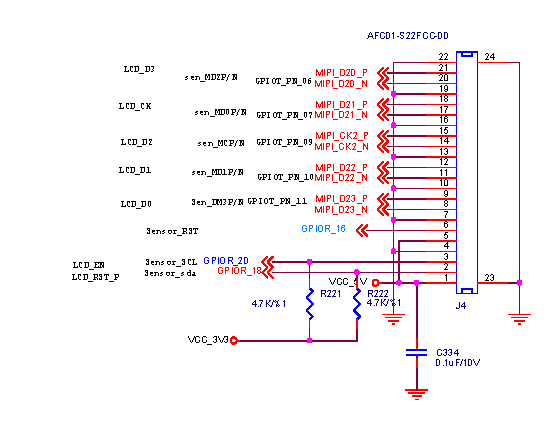
\includegraphics[width=.91\linewidth,height=2.7cm,keepaspectratio,trim={70bp 9bp 7bp 114bp},clip]{figures/camera_j4.pdf}\\[-1pt]
{\small (a) J4控制线与上拉电阻}
\end{minipage}\hfill
\begin{minipage}[b]{.46\linewidth}\centering
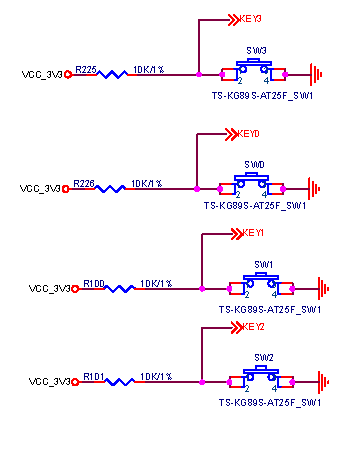
\includegraphics[width=.91\linewidth,height=2.7cm,keepaspectratio,trim={0bp 163bp 0bp 0bp},clip]{figures/keys_circuit.pdf}\\[-1pt]
{\small (b) KEY3按下接地}
\end{minipage}
\caption{摄像头控制与按键输入的局部电路，摘自Ti60 V4板级原理图\cite{board}。}\label{fig:hw-small}
\end{figure}

\subsection{软件系统与模块设计}
软件分为离线训练程序和板上控制程序。训练程序将十组参数导出为整数参数包，随配置文件进入板上ROM。板上的Sapphire RV32IM运行C固件，在32\,KiB片内RAM中维护当前风格、视图请求和手势模板。C程序经APB读写设备寄存器，像素则经AXI直接在DDR与专用RTL模块之间传输。这一分工使处理器可以在卷积计算期间继续响应按键和分析手势快照。

\begin{table}[H]\centering\small
\caption{板上视频软件与专用逻辑的模块接口}\label{tab:swroles}
\begin{tabularx}{\linewidth}{@{}p{.23\linewidth}p{.32\linewidth}X@{}}\toprule
模块、执行位置 & 主要输入 & 输出及下游使用方式\\\midrule
设备与风格控制（C） & 目标风格、采集及引擎状态、ROM参数 & I\textsuperscript{2}C配置，APB参数地址/数据，作业启动。PLIC IRQ16返回作业事件。\\
采集与源帧管理（RTL） & 四lane PPI字节及状态，RAW行与帧边界 & RGB565源帧。给作业控制器提供最新完整帧号和可锁定的槽。\\
分条DMA与卷积核（RTL） & 源、目的槽地址，已加载权重，本次视图 & 结果帧及完成/错误信号。完成条件包含最后一笔DDR写响应。\\
显示读取与叠加（RTL） & 待提交槽号、帧号、视图和风格，C/I等状态 & 在消隐期确认切换，输出同步、数据有效和RGB，驱动TMDS。\\
手势交互（RTL＋C） & 有效原图区域、模式、按键，带序号的64×64快照 & C程序输出候选与确认进度，确认后向控制器提交目标风格。\\\bottomrule
\end{tabularx}\end{table}

图\ref{fig:frame_messages}以一次风格作业说明控制关系。软件可以在收到计算完成中断后调度下一幅图，而一幅图究竟何时出现在屏上，由显示端的消隐确认决定。因此屏上的风格编号取自前台帧的元数据。
\begin{figure}[H]\centering
\begin{tikzpicture}[x=1cm,y=.72cm,font=\small,
lane/.style={draw=navy!65,fill=pale,rounded corners=2pt,minimum width=2.55cm,minimum height=.58cm},
msg/.style={-{Stealth[length=2mm]},draw=teal,thick},
lbl/.style={midway,above,inner sep=1pt,font=\footnotesize}]
\foreach \x/\t in {0/RISC-V固件,3.55/帧与作业控制,7.1/CNN及DMA,10.65/显示读取} {
 \node[lane] at (\x,0){\t};\draw[navy!35,dashed] (\x,-.45)--(\x,-6.3);}
\draw[msg] (0,-.95)--node[lbl]{参数就绪，启动作业}(3.55,-.95);
\draw[msg] (3.55,-1.95)--node[lbl]{锁住源帧，指定输出槽}(7.1,-1.95);
\draw[msg] (7.1,-2.95)--node[lbl]{计算结束，最后B已返回}(3.55,-2.95);
\draw[msg] (3.55,-3.9)--node[lbl]{完成事件经PLIC通知}(0,-3.9);
\draw[msg] (3.55,-4.8)--node[lbl]{提交完整结果及帧号}(10.65,-4.8);
\draw[msg] (10.65,-5.8)--node[lbl]{安全消隐确认，释放旧前台}(3.55,-5.8);
\end{tikzpicture}
\caption{一次风格作业的关键事件。从上往下阅读。中断和显示提交使用各自的握手，图中行距不表示时间间隔。}\label{fig:frame_messages}
\end{figure}

\subsubsection{采集与源帧管理}
固件释放模组复位，通过I\textsuperscript{2}C读取寄存器\sig{0x3107/0x3108}，确认器件ID为\sig{0xCD6B}，设置并读回1920×1080输出尺寸，再根据实际帧长限制曝光。摄像头开流后，D-PHY输出的四路字节、有效位和同步状态被打成一条44位记录。深度为512的异步FIFO将整条记录从接收字节时钟域送入100\,MHz的用户接口域。即使摄像头在低功耗间隔暂停字节时钟，同一批字节与其状态仍能对应。

CSI解析模块核验包头ECC、行负载长度及CRC。1920个RAW10样本每行占2400字节，每五字节还原四个十位值。Bayer模块取样本高八位，以两条行缓存形成$3\times3$邻域。例如在蓝色像素处，中心值保留为B，四个正交邻点的平均值为G，四个对角邻点的平均值为R。缩放逻辑沿横纵两轴按$0,1,3,4,\ldots$选取插值后的像素，得到1280×720图像。每个有效输出拍含两个RGB565像素，较左像素占低16位。

\sig{camera_pack_720}将四拍双像素组成一个128位DDR词，并携带源帧号和17位字索引。行跨度为2560字节，故像素$(x,y)$的地址为$A_{\rm src}+2560y+2x$。一帧共115200个词，占1843200字节。帧尾记录、连续词数和最后的AXI写响应均有效时，源池才发布这幅图。格式错误或写响应错误会使整帧作废。

源池的三个槽从4、6、8\,MiB起始。\sig{source_frame_pool}在作业领取最新好帧时锁住其槽，采集端选择另一个空槽继续写。当新帧到来而上一幅完整帧仍未被领取，池中以新帧替换它并累计跳过数。该计数与摄像头传输坏帧分开，可用于区分采集质量和推理是否跟得上输入。

\subsubsection{风格调度与分条计算}
假设当前正显示梵高，操作者按键选择水墨。按键模块只更新请求槽号。固件在引擎空闲时，从APB基址\sig{0xF8100000}加上$\mathtt{0x4000}+736s$的位置读取槽$s$的参数，按层写入权重、偏置和移位。跨域邮箱保持地址和数据，直到166.667\,MHz的CNN域完成写入并应答。处理器核对216项配置后提交新的已加载槽号。当完整源帧可用时再启动作业。若中途又收到操作，当前作业使用启动时锁存的风格，后续作业处理最新请求。

整幅六通道特征图占$1280\times720\times6$字节，远大于处理一个局部窗口所需的存储。引擎沿宽度划分四条，每条交付中央320列，并在两侧各保留16列邻域供卷积读取。图\ref{fig:tilegeometry}以第二条为例。它输出全图第320--639列，输入窗口横跨304--655列，同一段边缘可以由相邻两条共享。宽度352列的行历史在四条之间复用。

\begin{figure}[H]\centering
\begin{tikzpicture}[x=1cm,y=1cm,font=\small]
\foreach \i/\a/\b in {0/0/319,1/320/639,2/640/959,3/960/1279}{
 \pgfmathsetmacro{\lx}{3*\i}
 \ifnum\i=1 \fill[teal!22] (\lx,0) rectangle ++(3,.57);\else\fill[pale] (\lx,0) rectangle ++(3,.57);\fi
 \draw[navy!65] (\lx,0) rectangle ++(3,.57);
 \node at (\lx+1.5,.285){\a--\b};}
\node[anchor=west,font=\footnotesize] at (0,.89){全图横坐标（列），每条均处理720行};
\draw[navy!55,dashed] (3,0)--(2.2,-.7);\draw[navy!55,dashed] (6,0)--(9.8,-.7);
\filldraw[fill=orange!16,draw=navy!70] (0,-1.35) rectangle (2.2,-.7);
\filldraw[fill=teal!22,draw=navy!70] (2.2,-1.35) rectangle (9.8,-.7);
\filldraw[fill=orange!16,draw=navy!70] (9.8,-1.35) rectangle (12,-.7);
\node at (1.1,-1.02){304--319};\node at (6,-1.02){320--639};\node at (10.9,-1.02){640--655};
\node[font=\footnotesize] at (1.1,-1.63){邻域16列};\node[font=\footnotesize] at (6,-1.63){写回DDR的320列};\node[font=\footnotesize] at (10.9,-1.63){邻域16列};
\end{tikzpicture}
\caption{四条带覆盖全幅图像。下栏展开第二条，邻域宽度为便于阅读而放大。四条合计写回921600个独立像素。}\label{fig:tilegeometry}
\end{figure}

感受野半径为15像素，16列重叠足以让中央区域取得完整邻域。各卷积层以全图边缘为镜像边界，分条接缝保留真实邻点，因而物体跨过接缝时仍有连续的笔触。DW用行缓存和三组列存储提供空间取样。PW用两条输出通道并行运算，由四组上下文交叠处理不同像素，结果按输入顺序送往下一层。原RGB经FIFO与头部增量对齐后相加，输入停顿或输出背压时两条支路保持对应。

分条引擎\sig{video_tile_engine_async}每次通过DMA突发读16个128位词，将256字节缓存到片上。卷积结果每八个像素拼成一个128位写词，两组写缓冲交替拼包和等待总线应答。必须等四条的有效列写完并收到最后一个写响应，才将结果加入输出队列。三个输出槽位于0、2、10\,MiB，可分别保存正在计算的帧、待提交的帧与正在扫描的前台帧。完成事件经PLIC通知固件，处理器可在显示端等待消隐期间调度下一幅图。

\subsubsection{显示合成与状态叠加}
原图视图把源帧复制到输出槽，风格视图写入卷积结果。左右对比在写回前完成合成。对每一个输出坐标，逻辑以全局$x<640$选择对齐后的原RGB，其余列选择风格结果，合成后的整帧共用一个源帧号。这样，即使镜头前的手在运动，中线两侧仍对应同一次采集。每个输出槽同时保存视图与风格编号。

显示读取模块\sig{frame_reader}通过AXI把前台数据送入像素FIFO。像素端以74.25\,MHz产生每行1650拍、每帧750行的扫描时序，有效区为1280×720。结果队列提交新槽时，读取模块排空旧地址的在途读请求，并等待FIFO复位在读写两个时钟域完成。它在有效区开始前保留一行余量，确认仍处于消隐窗口才应答换帧。错过窗口就等待下一次消隐，避免同一次屏幕扫描混入两幅画面。

信息层按像素坐标叠加文字和手势框。C统计一秒内采集模块发布的好帧，I统计一秒内完成的神经网络作业，H60对应固定的HDMI扫描设置。显示器重复扫描前台时，I保持实际作业计数。S随新前台一同更新，因此可以用它判断风格何时真正出现。KEY3只切换文字和青框的可见性。USB串口以CAM7记录输出帧数、作业周期和错误计数，供连续测量使用。

\subsubsection{按键与手势交互}
KEY0在原图、风格图、左原右风格三种视图间循环，KEY1和KEY2在十个风格槽间前后选择。四路低有效按键经过两级同步和约10\,ms消抖，每次按下仅产生一次操作。手势与按键共用风格请求入口，区别在于手势先经过图像分类和持续时间判定。

当请求视图与前台一致，且处于原图或对比模式时，系统允许手势采样。采样器从原图左侧640×640的青框区域取样。采样器在横纵方向每10个像素取一点，得到64×64 RGB565快照。只有4096个采样点及好帧帧尾均已到达，处理器才可读取。快照附带序号和界面状态标识，同一张快照只用于一次判定。此旁路占8\,KiB，可以在主视频保持720p时独立使用。

首次使用个人手势时，按住KEY1与KEY2约一秒进入学习，在空框内采三张背景，再为每类手势各录四张。处理器先补偿整体亮度变化，再对背景差分结果保留最大连通区域，用亮度的第5和第95百分位规范化手形。每张样本提取192维特征，包括64维梯度方向、64维局部灰度及64维轮廓密度。软件比较正向和镜像的模板距离，并以最优距离及其与次优类别的间隔拒绝歧义。模板存于RAM，重新配置后须重新录入。

\begin{table}[H]\centering\small
\caption{数字手势与风格槽的对应关系。数字0与未检测到手势分别编码。}
\begin{tabularx}{\linewidth}{@{}clXclX@{}}\toprule
槽 & 风格 & 手形 & 槽 & 风格 & 手形\\\midrule
0 & 梵高厚涂 & 五指弯曲围成O形 & 5 & 阿什维尔抽象 & 五指张开\\
1 & 浮世绘 & 食指 & 6 & 形体对比 & 拇指、小指\\
2 & 彩色剪纸 & 食指、中指 & 7 & 蒙德里安几何 & 拇指、食指、小指\\
3 & 复古漫画 & 中指、无名指、小指 & 8 & 彩色马赛克 & 拇指、食指\\
4 & 竹林水墨 & 除拇指外四指 & 9 & 雨夜厚涂 & 食指弯钩\\\bottomrule
\end{tabularx}\end{table}

运行时每约333\,ms抓取一幅新快照，三张中的多数结果形成一次决定。第一个有效决定开启计时，约在第0、1、2、3、4秒连续得到同一数字，且实际经过四个完整秒后才提交。候选变化、界面切换或快照过期都会清除累计进度。原图确认后自动进入风格图，对比视图确认后仍保留左右两侧。图\ref{fig:gesture-time}用数字2示意一次成功识别。
\begin{figure}[H]\centering
\begin{tikzpicture}[x=2.1cm,y=1cm,font=\small]
\draw[-{Stealth},navy] (-.35,0)--(4.95,0);
\foreach \i in {0,1,2,3,4}{
 \draw[navy] (\i,-.07)--(\i,.07);\fill[teal] (\i,0) circle(2.1pt);
 \node[above] at (\i,.12){G2};\node[below] at (\i,-.12){P\i};}
\node[anchor=west,font=\footnotesize] at (4.18,.42){提交槽2};
\node[font=\footnotesize] at (2,-.85){相邻决定约间隔1秒，每个决定使用三张新快照};
\end{tikzpicture}
\caption{手势的四秒确认。首个决定记为P0，第五个同类决定且经过四秒可提交。前台实际更新后显示S2。}\label{fig:gesture-time}
\end{figure}

\Needspace{7\baselineskip}
\section{完成情况及性能参数}
\subsection{整体介绍}
在原图界面伸出食指和中指，系统确认手势后选择第2号风格，HDMI屏自动显示彩色剪纸。回到左右对比界面，移动镜头前的物体，同一帧的轮廓可以横跨中线连续显示。

\subsection{赛题要求与完成情况}
系统在Ti60上完成了从摄像头原始像素到风格画面的处理。SC431HAI输出1920×1080 RAW10，FPGA将其转换为1280×720 RGB565图像。卷积网络在这一分辨率上逐像素生成风格结果，HDMI提供全屏原图、全屏风格和左原右风格三种视图。

\begin{table}[H]\centering\small
\caption{实时绘画赛题的设计要求与系统实现}\label{tab:contest}
\begin{tabularx}{\linewidth}{@{}p{.20\linewidth}p{.31\linewidth}X@{}}\toprule
功能 & 赛题要求 & 系统实现及已有结果\\\midrule
采集与预处理 & MIPI CSI-2，至少640×480、30帧/秒 & 四通道接收RAW10，完成包校验、Bayer插值及720p缩放。每发布一幅好帧更新采集计数。\\
外部帧缓存 & 双缓冲保存完整帧，保障采集连续 & DDR3设置三个原图槽、三个输出槽。采集、推理和显示分别持有所用帧，记录跳帧、坏帧和欠载。\\
卷积加速与控制 & 3×3或5×5卷积、激活和归一化，总线读写DDR，RISC-V调度 & FPGA实现3×3深度卷积、1×1通道混合和饱和激活，BN折叠入卷积。RISC-V配置摄像头、加载参数，管理作业与完成中断。\\
显示与对比 & 720p60或1080p30，原画对比及FPS叠加 & HDMI使用74.25\,MHz像素时钟输出720p60。左右两侧取自同一源帧，屏显C、I分别给出采集和推理帧率。\\
处理速度 & 基础目标为640×480稳定超过15帧/秒，高阶目标为720p达到30帧/秒 & 720p槽0对比模式的CNN/DMA整帧仿真处理921600像素，耗时25.585\,ms，折合39.085帧/秒。\\
多风格与模型规模 & 至少两种风格，切换低于100\,ms且不丢帧，模型小于500\,KB & 十组风格共用一个加速器。每风格567个可训练参数、396个卷积系数，十组部署参数共7360字节。支持按键及手势选画。\\\bottomrule
\end{tabularx}\end{table}
整机持续帧率、丢帧数和按键切换延迟尚待现场实测。

\subsection{工程成果}
\subsubsection{机械与电路成果}
摄像头以排线连接J4，HDMI输出端连接显示器，USB串口连接测量主机。配置审查覆盖79个物理端口及12组Bank，逐项核对信号方向、电压域和DDR数据选通。实物连接与运行画面在本章实拍栏中记录。

\subsubsection{软件成果}
十个风格分支共5670个可训练参数。离线程序将各分支导出为整数参数包，板上10588字节的RISC-V固件负责选择参数、调度推理和处理手势请求。CAM7串口输出帧数、作业周期和交互状态。

\subsection{资源占用与处理性能}
布局布线后，整机使用142个DSP和230块RAM10。DSP承担卷积乘加，RAM10用于行缓存、像素队列、处理器存储和手势快照。图\ref{fig:utilization}给出三类主要资源的占比。逻辑资源XLR的使用率最高，为97.06\%。整机使用29702个寄存器和32898个查找表，I3时序模型下最小建立、保持余量分别为+0.108\,ns和+0.026\,ns。
\begin{figure}[H]\centering
\begin{tikzpicture}[x=1cm,y=.80cm,font=\small]
\foreach \y/\name/\used/\total/\pc in {2/RAM10/230/256/89.84,1/DSP/142/160/88.75,0/XLR/59011/60800/97.06}{
 \node[anchor=east] at (-.17,\y+.23){\name};
 \fill[navy!9] (0,\y) rectangle (7.0,\y+.48);
 \fill[teal!85] (0,\y) rectangle ({.07*\pc},\y+.48);
 \node[anchor=west,font=\footnotesize] at (7.13,\y+.23){\used\,/\,\total\quad(\pc\%)};
}
\node[anchor=west,font=\footnotesize] at (0,-.42){已用资源占器件总量的比例};
\end{tikzpicture}
\caption{Ti60F225I3布局布线后的资源占用。十个风格槽共享同一组卷积算子和行缓存。}\label{fig:utilization}
\end{figure}

梵高风格的完整720p对比帧在CNN/DMA仿真中用时2558528个100\,MHz时钟周期。921600个输出像素与整数参考逐点一致。该时间包含条带运算、读写背压和最后一次写响应，对应每帧25.585\,ms。板上运行时，信息层从采集与推理计数器取数，在消隐期同步到显示端，如图\ref{fig:rates-ui}所示。

\begin{figure}[H]\centering
\begin{tikzpicture}[x=1cm,y=1cm,font=\small,
 stage/.style={draw=navy!65,rounded corners=2pt,fill=pale,align=center,inner sep=4pt},
 arrow/.style={-{Stealth[length=2mm]},draw=teal,thick}]
\node[stage,minimum width=3.65cm] (cap) at (0,1.12) {源帧成功发布};
\node[stage,minimum width=3.65cm] (cnn) at (0,0) {风格帧写回完成};
\node[stage] (dc) at (4.1,1.12) {采集计数每秒增量};
\node[stage] (di) at (4.1,0) {推理计数每秒增量};
\node[stage,fill=teal!12] (c) at (7.95,1.12) {屏显 C};
\node[stage,fill=teal!12] (i) at (7.95,0) {屏显 I};
\draw[arrow] (cap)--(dc);\draw[arrow] (cnn)--(di);\draw[arrow] (dc)--(c);\draw[arrow] (di)--(i);
\node[stage,minimum width=3.65cm] (clock) at (0,-1.18) {像素时钟74.25\,MHz};
\node[stage] (scan) at (4.1,-1.18) {每帧$1650\times750$拍};
\node[stage,fill=orange!13] (h) at (7.95,-1.18) {屏显 H60};
\draw[arrow] (clock)--(scan);\draw[arrow] (scan)--(h);
\end{tikzpicture}
\caption{屏幕三项速率的来源。C与I分别由完整采集和神经作业完成事件得到，H60由视频扫描时序确定。}\label{fig:rates-ui}
\end{figure}

十组参数均通过小尺寸RTL与映射算子逐值核对。RISC-V固件仿真覆盖十槽加载，共完成2160项参数写入。手势全流程验证依次输入3张空背景、40张个人模板和15张识别快照，经过4.08秒的确认窗口后，固件提交对应风格请求。

\clearpage
\subsection{十风格训练效果}
两张公共领域作品《蒙娜丽莎》和《戴珍珠耳环的少女》分别由来源页面获取\cite{mona,pearl}，在十组参数上保持相同输入，便于比较风格差异。每张原作按比例缩至高720像素，两侧反射补边为1280×720后量化RGB565，再运行当前最终整数模型；下图仅裁出原画有效区域，不改变模型输出颜色或锐度。

以下各图从左至右依次为《蒙娜丽莎》原图与转换图、《戴珍珠耳环的少女》原图与转换图。观察同一处发丝、衣褶和背景，可以比较不同参数对轮廓、明暗与短笔触的处理。


\begin{figure}[H]\centering
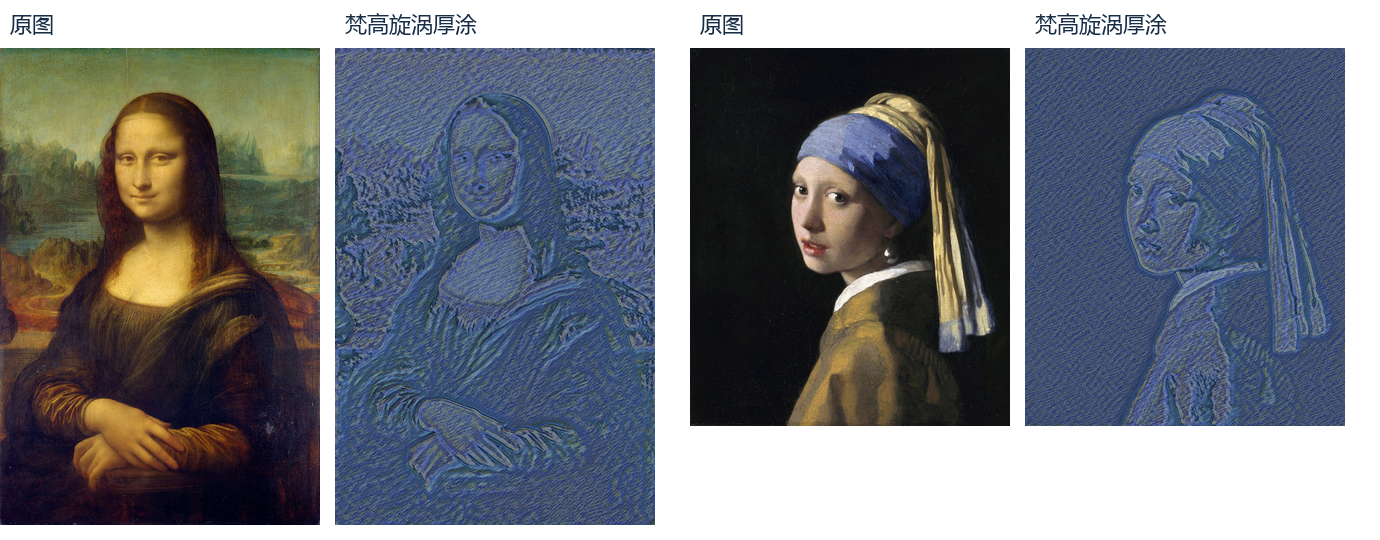
\includegraphics[width=\linewidth]{assets/comparisons/style_00_pairs.png}
\caption{槽0 梵高旋涡厚涂}
\end{figure}
\begin{figure}[H]\centering
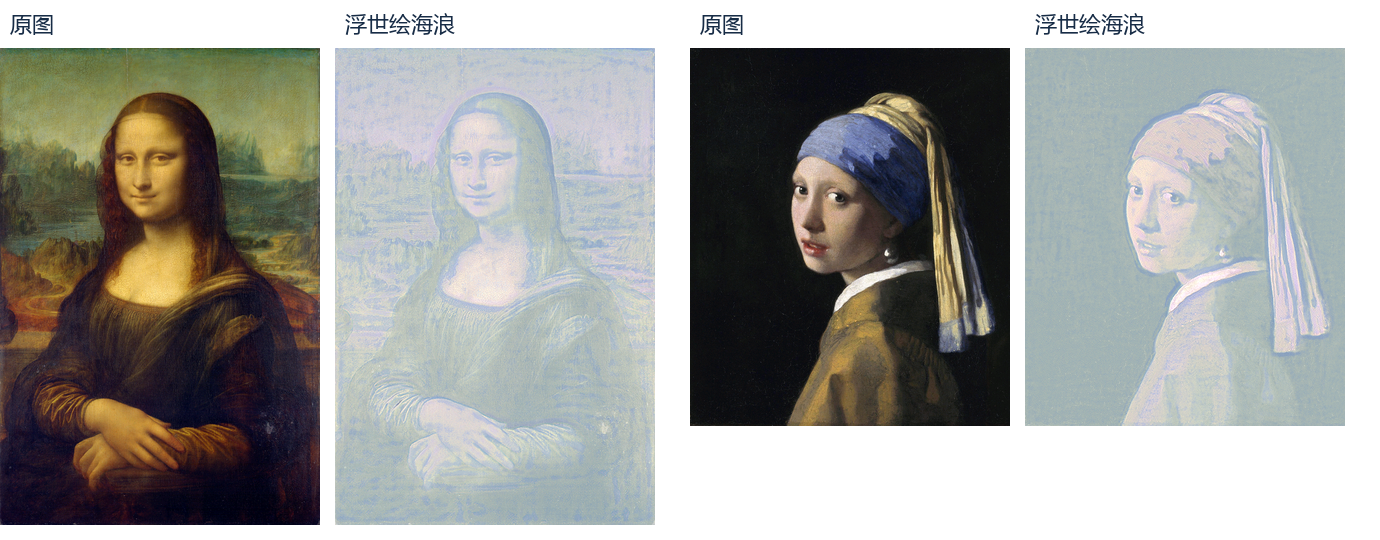
\includegraphics[width=\linewidth]{assets/comparisons/style_01_pairs.png}
\caption{槽1 浮世绘海浪}
\end{figure}

\clearpage
\begin{figure}[H]\centering
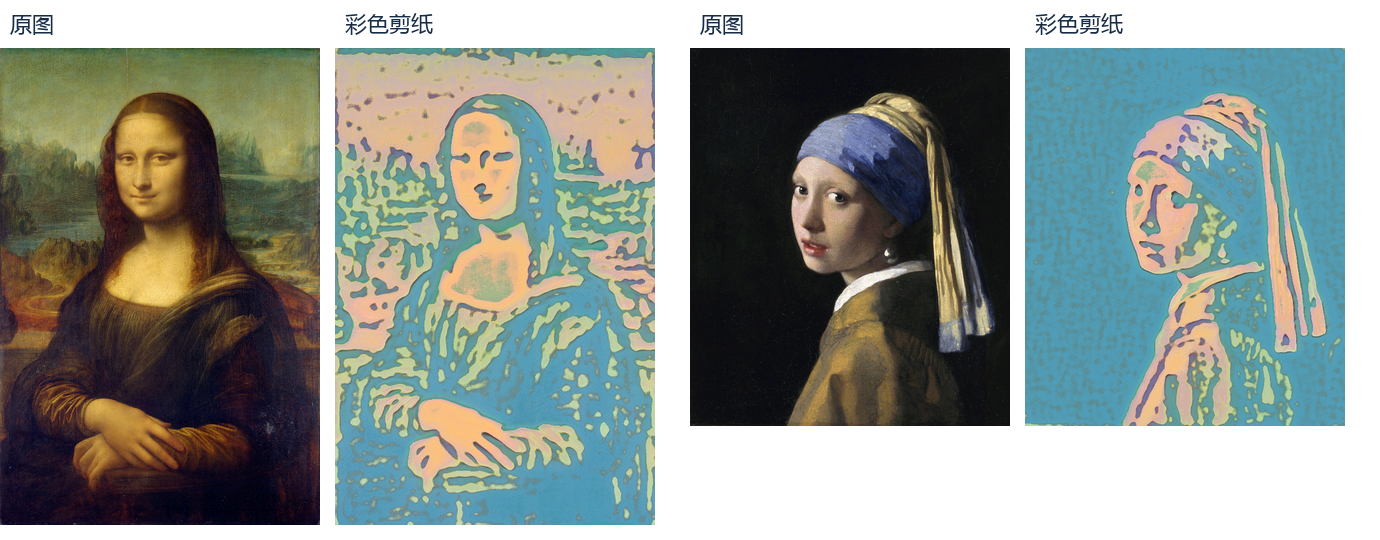
\includegraphics[width=\linewidth]{assets/comparisons/style_02_pairs.png}
\caption{槽2 彩色剪纸}
\end{figure}
\begin{figure}[H]\centering
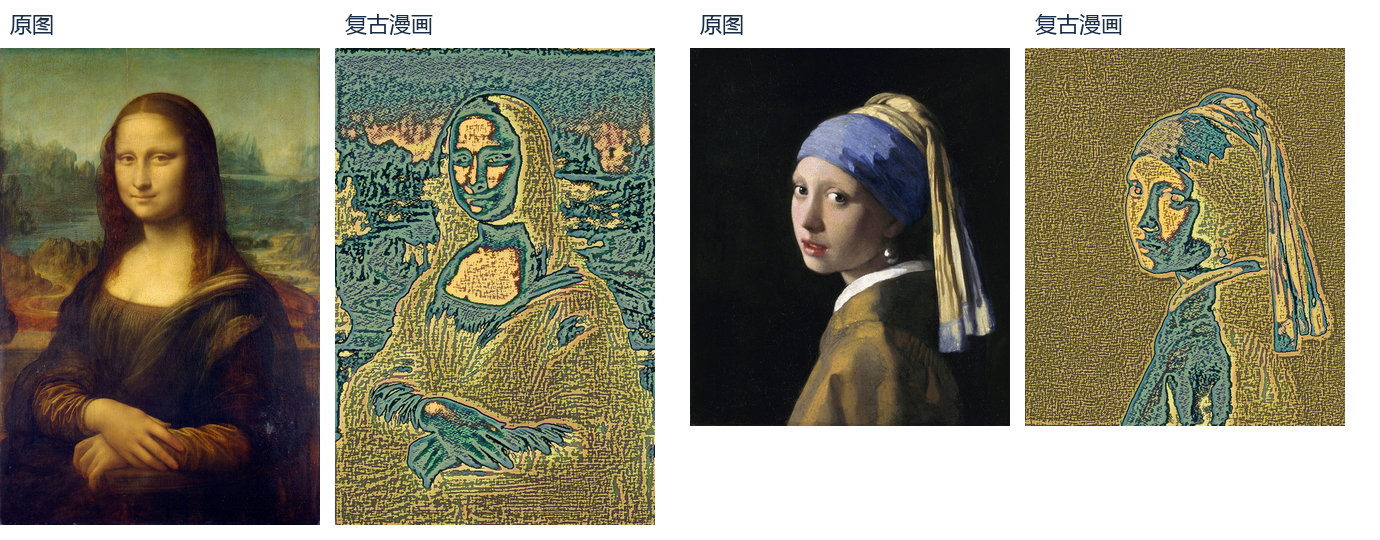
\includegraphics[width=\linewidth]{assets/comparisons/style_03_pairs.png}
\caption{槽3 复古漫画}
\end{figure}

\clearpage
\begin{figure}[H]\centering
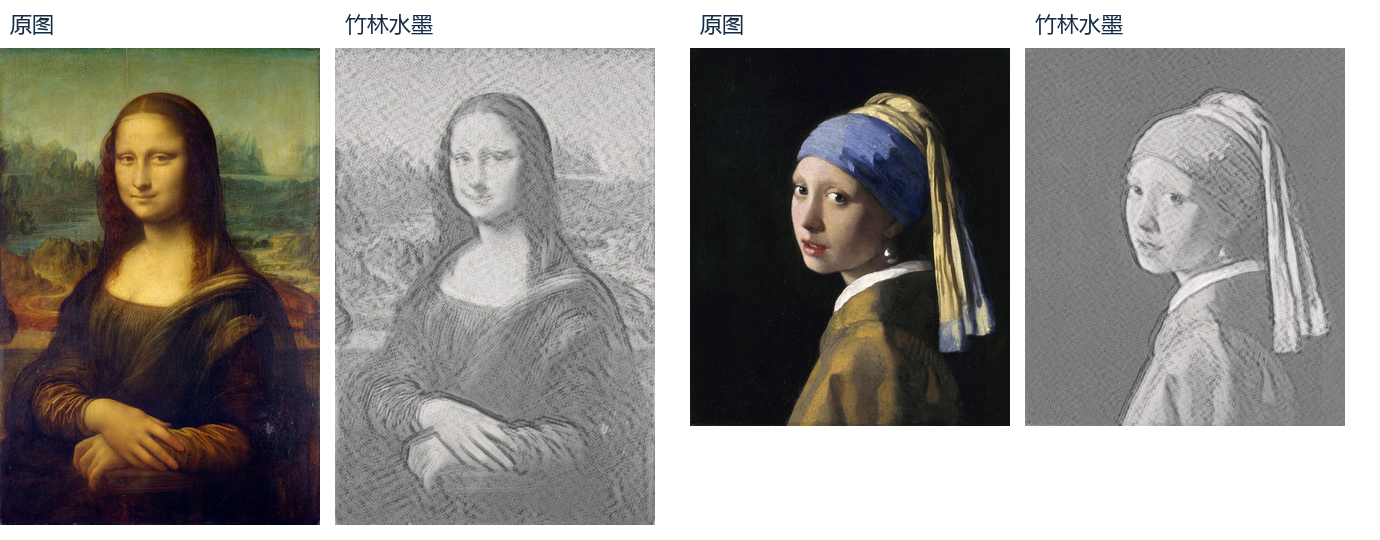
\includegraphics[width=\linewidth]{assets/comparisons/style_04_pairs.png}
\caption{槽4 竹林水墨}
\end{figure}
\begin{figure}[H]\centering
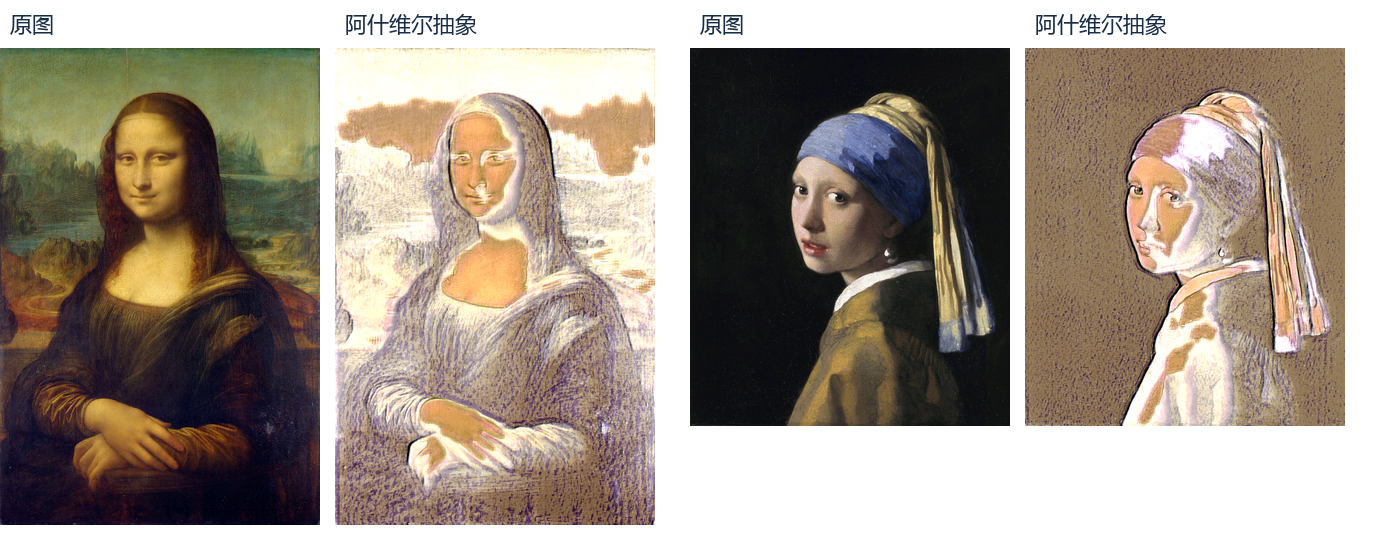
\includegraphics[width=\linewidth]{assets/comparisons/style_05_pairs.png}
\caption{槽5 阿什维尔抽象}
\end{figure}

\clearpage
\begin{figure}[H]\centering
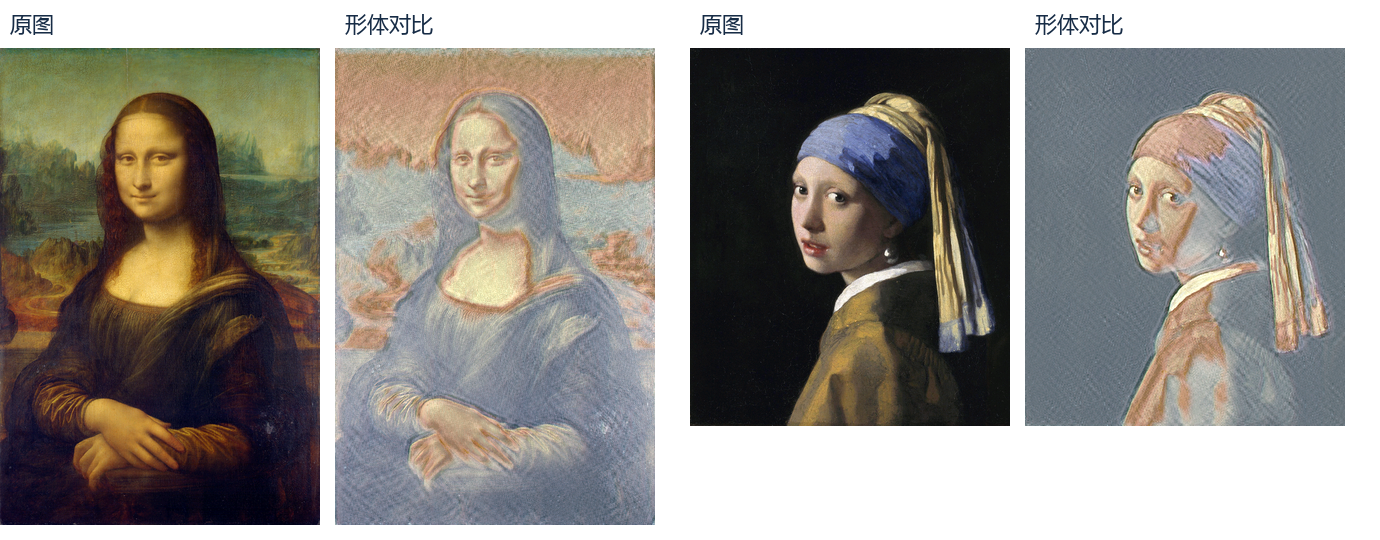
\includegraphics[width=\linewidth]{assets/comparisons/style_06_pairs.png}
\caption{槽6 形体对比}
\end{figure}
\begin{figure}[H]\centering
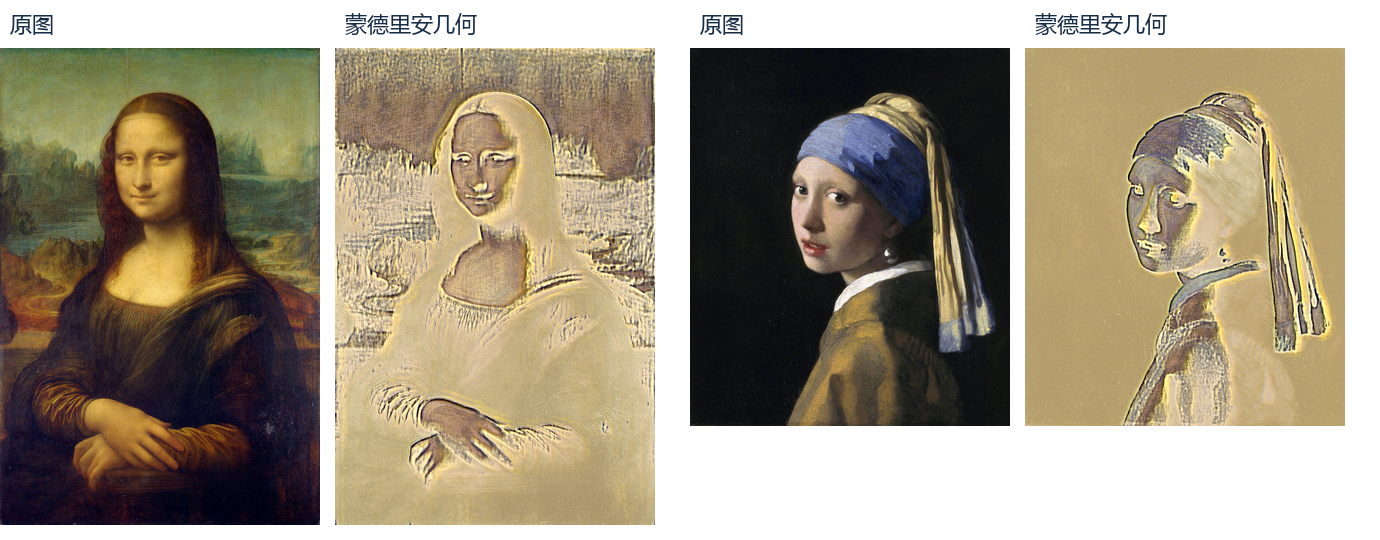
\includegraphics[width=\linewidth]{assets/comparisons/style_07_pairs.png}
\caption{槽7 蒙德里安几何}
\end{figure}

\clearpage
\begin{figure}[H]\centering
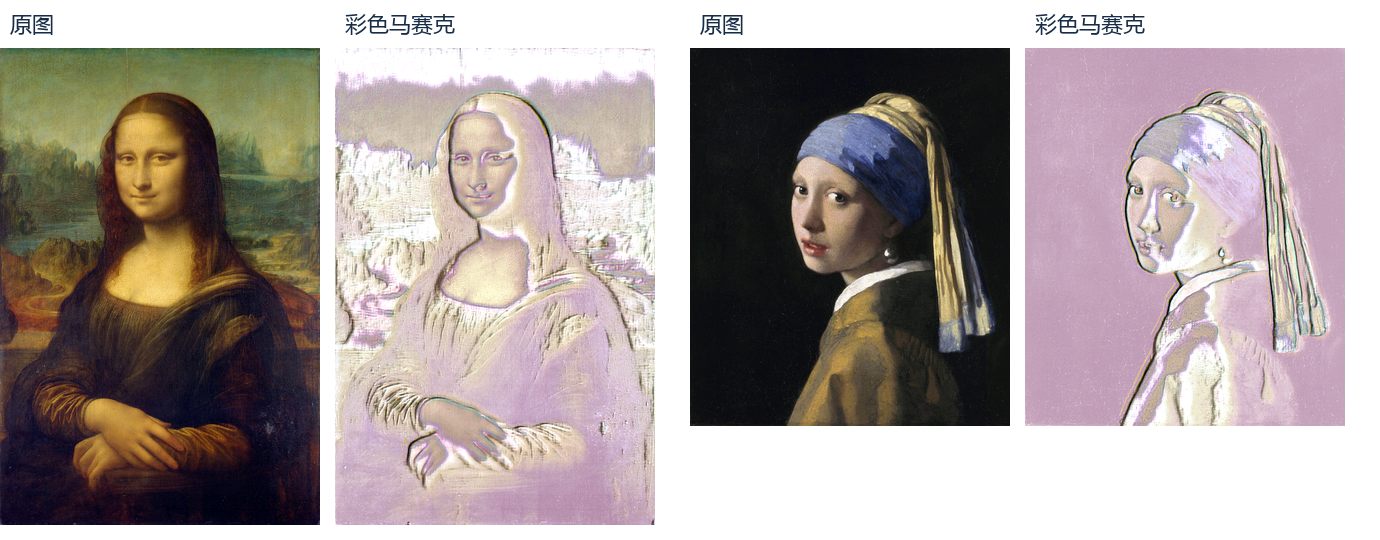
\includegraphics[width=\linewidth]{assets/comparisons/style_08_pairs.png}
\caption{槽8 彩色马赛克}
\end{figure}
\begin{figure}[H]\centering
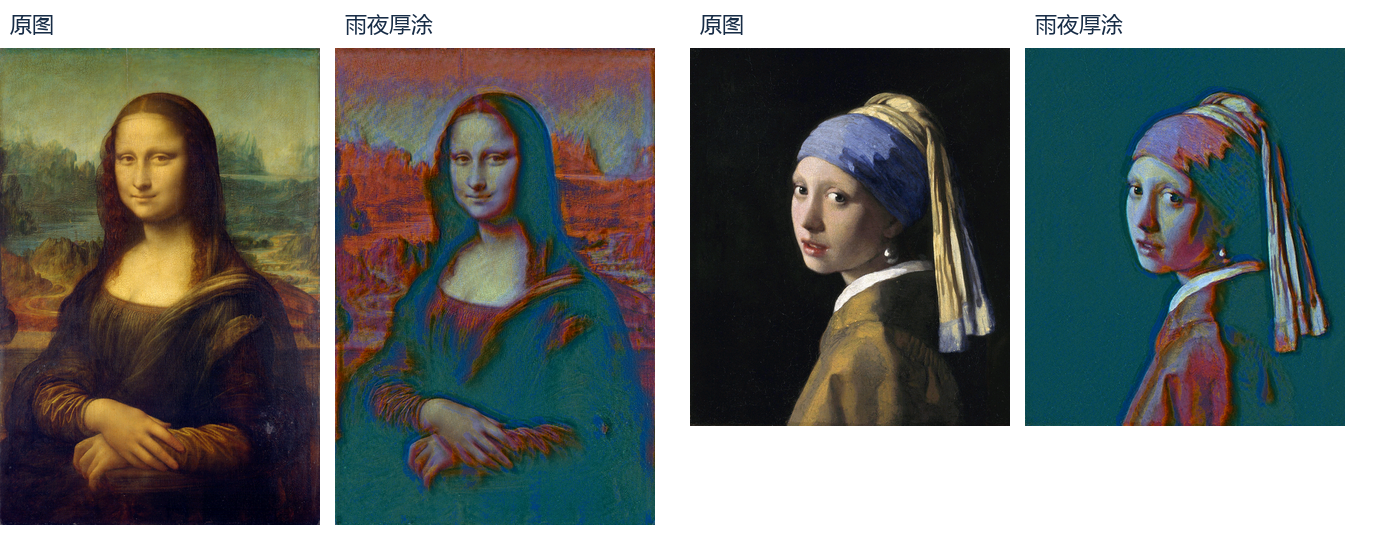
\includegraphics[width=\linewidth]{assets/comparisons/style_09_pairs.png}
\caption{槽9 雨夜厚涂}
\end{figure}

\clearpage
\subsection{实物展示与读数}
\newcommand{\fieldshot}[3]{\begin{minipage}[t]{.48\linewidth}\centering
\IfFileExists{assets/field/#1.jpg}{\includegraphics[width=\linewidth,height=.135\textheight,keepaspectratio]{assets/field/#1.jpg}}{\IfFileExists{assets/field/#1.png}{\includegraphics[width=\linewidth,height=.135\textheight,keepaspectratio]{assets/field/#1.png}}{\fbox{\parbox[c][.122\textheight][c]{.91\linewidth}{\centering\textcolor{teal}{\textbf{#1}}\par\small 待补实拍}}}}
\par\smallskip{\small\bfseries #2}\par{\footnotesize #3}\end{minipage}}
\noindent\fieldshot{P01}{原图与装置}{同框保留SC431HAI、开发板、HDMI屏及原场景。}\hfill
\fieldshot{P02}{风格图}{固定机位，记录风格S和一处可辨识的纹理。}
\par\medskip\noindent\fieldshot{P03}{同源左右对比}{让物体横跨中线，观察两侧轮廓与运动是否衔接。}\hfill
\fieldshot{P04}{手势确认}{完整的手置于框中，记录候选G及进度P；视频保留确认过程。}
\par\medskip\noindent\fieldshot{P05}{UI开启}{记录屏上完整字段及手势确认后的前台槽S。}\hfill
\fieldshot{P06}{UI关闭}{同一视图按KEY3，以相同机位记录干净画面。}
\par\medskip
\noindent C为一秒内发布的好采集帧数，I为完成的新风格推理帧数，H60表示配置的HDMI刷新率。G为投票后的候选数字，短横线表示暂无候选。P为已经持续的完整秒数，范围0--4。S为已经提交到前台的风格槽号。录入时，L显示当前标签，A显示已经接受的样本数量。青框标出镜头中采样手势的区域。
\clearpage
\blocktitle{名画输入的实屏对照}
\noindent\fieldshot{P07}{《蒙娜丽莎》}{十风格摄像头版，镜头采集原画，KEY3关闭UI。}\hfill
\fieldshot{P08}{《戴珍珠耳环的少女》}{十风格摄像头版，固定机位，记录实际风格槽。}
\par\bigskip
\noindent\fieldshot{U01}{串口输入《蒙娜丽莎》}{UART四风格验证工程，上传源图后在板上转换。}\hfill
\fieldshot{U02}{串口输入《戴珍珠耳环的少女》}{UART四风格验证工程，记录板上按键选择。}
\par\bigskip
摄像头图组包含光照、镜头曝光、白平衡与显示器再拍摄的影响。串口图组采用确定的RGB565输入和四风格模型。两条路径分别标记，便于说明色差和纹理差异来自哪一环节。

\blocktitle{板端运行记录}
采集与推理按完整帧计数。切换延迟取按键消抖完成至新风格前台生效的时间差。
\begin{center}\small\begin{tabularx}{\linewidth}{@{}p{.36\linewidth}XX@{}}\toprule
测量项 & 槽0风格图 & 槽4左右对比\\\midrule
时间窗 / 好采集帧增量 & 待测 & 待测\\
推理FPS均值 / 最低一秒 & 待测 & 待测\\
跳过源帧 / 坏帧 / 显示欠载 & 待测 & 待测\\
风格切换延迟 / 样本数 & 待测 & 待测\\\bottomrule
\end{tabularx}\end{center}

\clearpage
\section{总结}
\subsection{可拓展之处}
预期实现风格权重在线下载：主机发送带模型版本、层结构、长度及CRC的参数包，先写入非活动存储区；RISC-V完成边界、位宽与完整性检查，等待引擎空闲后装载并原子切换，失败保留旧模型。当前仅实现从预置ROM加载，不宣称已有外部在线更新。另将继续补足十手势真人样本、改善弱光前景提取，并完成持续30fps实测及功耗、温升评估。

\subsection{心得体会}
本项目的主要难点是画质、存储、计算和交互共同约束下的系统一致性。减少参数并不必然降低全部资源；恢复全720p后，行缓存、访存和显示仍需处理完整像素。采用DW/PW和六通道降低运算量后，进一步的收益来自多上下文流水、列bank及总线重叠，不能只提高PLL频率。

训练方面，较强像素蒸馏会保留内容却削弱笔触，过强纹理又可能遮蔽物体。通过弱化像素回归、加入绘画Gram和局部纹理能量，当前梵高细笔触有所恢复，但有限感受野仍不能完成大范围语义重绘。评价应结合多内容图和真实摄像头，不能只看参考图或单张好例。

系统方面，完整EOF、最终DDR响应、输出槽元数据和安全换帧必须统一；任一环节提前发布都可能把算法问题与缓存撕裂混在一起。诊断计数使采集、计算和显示可分别观察，降低联调歧义。电气核对也必须以实际板卡原理图为依据，不能把DRC通过当成供电正确。

手势试验进一步说明了数据定义和真实泛化的重要性。用户的O形0、后三指3与拇指食指小指7并不等于数据集数字标签；自动标注也会把收拇指的手势认成7。四秒保持可以降低短时跳变，却无法消除持续误认。因此当前保留可解释的个人录入版本，未达标的通用模型不装进交付bit，后续需先补足正确数据和前景提取验证。

最后，交付不仅是bit文件，还需保留模型、整数参考、固件、工程配置和测量范围。本文将CAD与仿真结果、实际模型图及待完成实测分别说明，使后续更新能够沿着清楚的版本基线继续。

\clearpage
\section{参考文献}
\begingroup\small
\renewcommand{\section}[2]{}
\begin{thebibliography}{12}
\bibitem{gatys} Gatys L A, Ecker A S, Bethge M. A Neural Algorithm of Artistic Style. arXiv:1508.06576, 2015. \url{https://arxiv.org/abs/1508.06576}.
\bibitem{johnson} Johnson J, Alahi A, Fei-Fei L. Perceptual Losses for Real-Time Style Transfer and Super-Resolution. ECCV, 2016. \url{https://arxiv.org/abs/1603.08155}.
\bibitem{mobilenet} Howard A G, et al. MobileNets: Efficient Convolutional Neural Networks for Mobile Vision Applications. arXiv:1704.04861, 2017. \url{https://arxiv.org/abs/1704.04861}.
\bibitem{qat} Jacob B, et al. Quantization and Training of Neural Networks for Efficient Integer-Arithmetic-Only Inference. CVPR, 2018. \url{https://arxiv.org/abs/1712.05877}.
\bibitem{board} Ti60F225I3 DemoBoard V4原理图. \sig{TI60F225I3-V4_SCH-20261012（原理图）.pdf}, 2026.
\bibitem{sensor} 思特威. SC431HAI CMOS图像传感器数据手册 V1.1. 本地厂商资料.
\bibitem{mona} Leonardo da Vinci. Mona Lisa. C2RMF图像, Wikimedia Commons公共领域艺术品页面. 访问日期2026-11-03. \url{https://commons.wikimedia.org/wiki/File:Mona_Lisa,_by_Leonardo_da_Vinci,_from_C2RMF_retouched.jpg}.
\bibitem{pearl} Johannes Vermeer. Girl with a Pearl Earring. Wikimedia Commons公共领域艺术品页面. 访问日期2026-11-03. \url{https://commons.wikimedia.org/wiki/File:Girl_with_a_Pearl_Earring.jpg}.
\bibitem{evidence} 本项目签核记录. \sig{camera_art_ten_paint/build/720p/signoff.json}与\sig{final_review.json}, 2026-11-02; 本报告新增\sig{assets/comparisons/verification.json}, 2026-11-03.
\end{thebibliography}
\endgroup
\end{document}
